% Include a list of keywords after the abstract
\keywords{Vera C. Rubin Observatory,
Observatory Operations,
Performance Metrics,
Dashboard User Interface,
Operations Monitoring,
Nightly Performance}

\section{INTRODUCTION}
\label{sec:intro}  % \label{} allows reference to this section

As the Vera C. Rubin Observatory moves toward executing the ten-year Legacy Survey of Space
and Time (LSST)\cite{2019ApJ...873..111I}, multiple teams within the observatory have been working towards
formalizing the logging processes ahead of operations. Multiple teams within Rubin Observatory
have been working towards formalizing the logging processes ahead of operations.
These efforts have been characterized by the Observatory
Electronic Logging group of 2020, and further built upon by the Telescope and Site
software team in recent years. Multiple tools and workflows were created and integrated
into existing applications at the observatory to automate the creation and exploration of
the logs. These continual efforts culminate in a new team and focused effort towards
creating a platform to explore and contextualize both human- and computer- created logs.


\subsection{Observatory Electronic Logging}

In mid 2020 Rubin Observatory SIT-Com (System Integration, Testing, and COMmissioning)
formed a working group to map out the state of electronic logging ahead of commissioning.
This group set out to understand the logging tools and systems used at the observatory and
identify opportunities to unify the overall logging to increase communication between
teams and improve problem resolution. This group identified different types of logging
data important to each of the audiences: written observer remarks, telemetry from the
observatory control system stored in the Engineering and Facilities Database (EFD),
exposure metadata, engineering ticketing system (Jira), and others. They also identified
that relationships between this data add to the overall context and strength of each data
source.

There are many reasons to need an integrated logging platform such as efficient reporting
and addressing of technical faults, reporting observing efficiency statistics to our
funding agencies, and tracking how we spend our observing time. Knowing how our observing
time is impacted by planned/unplanned downtime and weather is critical to continued
operations. Interruptions to observing time and their resolutions need to be understood
and tracked for a single observing night, and over a larger time period.

The conclusion of this working group spawned multiple contributions to the logging
ecosystem at Rubin Observatory: Observer Logging Environment (OLE), where observers enter
live notes and link work tracking tickets into their control system interface
\cite{Aranda26}, and the Night Report where they summarize the observation night’s events.

\subsection{Telescope and Site Logging}

Despite the initial efforts and fruits of the logging working group of 2020, the landscape
of logging at Rubin Observatory in early 2024 was in a divided state. Differing teams had
developed bespoke logging metrics and platforms to monitor the performance of their system
at the observatory.

The observers had a view into each of the systems through the LSST Observer Visual
Environment (LOVE) as well as view their written logging through OLE\cite{Aranda26}. The
Telescope and Site software team had a view into the observatory control system and how
each component was running through their own logs. Sub-system owners had unique
chronograf dashboards (web application to visualize and query data from an InfluxDB instance)
measuring logs and telemetry from their systems, and people working offsite-outside of the summit created
interactive Jupyter notebooks run in Times Square in the Rubin Science Platform (RSP). Each technical group
had a slightly different focus and measure for how a ‘good night’ goes, and monitored
different slack channels, created their own daily/weekly/monthly summary reports, or used a
mixture of all the methods above.

Notable monitoring and logging systems had been created and widely used by summit staff to
this point, namely ROLEX (Rubin Observatory Log EXplorer) and RubinTV. ROLEX was a tool to
view observer remarks in time relation to observatory control system actions including scripts
run and telemetry created. RubinTV is a real-time application that analyzes and displays
data where summit staff can quickly view specific exposures and scientific metadata
plotted about the exposures and list these values for exposures taken within an observing
night \cite{RubinTV-Phalanx}. Each of these applications offered functionality that the
logging team could build upon or subsume into our unified monitoring platform. RubinTV will continue
to operate as a real-time monitoring application, and the Nightly Digest will be focused on providing
a more comprehensive and contextualized view of the night’s operations after the fact.

\section{The NightLog}
\label{sec:night log}

At this point, the logging team was assembled and tasked with revisiting the goals of a
previous logging working group. This initiated us to create a system with “the purpose of
exchanging information between the different technical teams and operations departments
during the commissioning and the operation of the observatory”\cite{LSE-490}. To get a
feel for the data landscape, demonstrate a clear prototype, and understand our
stakeholders use cases, the logging team created an interactive jupyter notebook running
within the RSP notebook aspect as our minimum viable product (MVP).
We hosted this MVP within the RSP’s Times Square, a service to publish jupyter notebooks
with project and data rights holders\cite{SQR-062}.

This MVP allowed the logging team to become familiar with these disparate logging data
sources and the types of metrics and visualizations our stakeholders were accustomed to
and preferential towards. Increasing stakeholder engagement with the MVP provided deeper
insight into project requirements and helped solidify alignment across the team.

When the MVP gained enough traction, the idea of a unified logging dashboard matured into
our current application: the Nightly Digest.



\section{The Nightly Digest}

Early 2025 we gathered resources and lessons learned from the MVP deployed in Times
Square. We better understood the audiences we were serving and
their use cases for logging and monitoring the operations of the telescope, during
commissioning and their monitoring vision through operations. Working with the in-kind
program and contributors from Astronomy Data and Computing Services (ADACS), we designed
an interactive dashboard composed of summary data and aggregated metrics spanning
different summit-based data sources to get a wide view of summit operations to engage and
serve our differing audiences. We call this dashboard and associated pages the Nightly
Digest.

\subsection{Architecture and Data Sources}

The Nightly Digest is deployed within a kubernetes platform managed by Phalanx, providing
access to data and services run at Rubin Observatory\cite{Phalanx-SPIE24, Phalanx-Docs}. The applications
deployed in Phalanx make up a large microservices architecture, including the Rubin
Science Platform, and spanning data access services, as well as the services that compose
the observatory control system. Nightly Digest’s integration into this larger
infrastructure enables us to take advantage of authentication, access control, load
balancing, and abstracts the infrastructure so our deployment is the same whether the Nightly
Digest is deployed on our summit infrastructure or on our US Data Facility (USDF).


The Nightly Digest’s front end displays a dashboard composed of applets with additional
pages expanding on different categories of information to drill-down into the details. The
front end architecture is based on a reactive component model using React, with TanStack
Table\cite{tanstack-table} and Recharts\cite{recharts} providing tabular and visualization infrastructure, and ShadCN/Tailwind
CSS\cite{shadcn-ui} supporting a consistent design system. Data retrieved from our back end are
transformed into interactive client-side views including synchronized plots, filtering
interfaces, and timeline-based operational summaries.

\subsubsection{Automated Data Sources}

We access control system telemetry from the \textbf{EFD}, a time-series based database backed by
InfluxDB\cite{SQR-068}. This data source provides detailed data including commands sent to components of the control
system, as well as data streams from sensors throughout the observatory. To access
exposures and their metadata, the Nightly Digest queries the \textbf{Consolidated Database (ConsDb)} \cite{DMTN-227}.
\textbf{ConsDB} is populated per exposure (rather than by timestamp) by summarizing telemetric data added to the \textbf{EFD} over the duration of an
exposure, or from other services including Rapid Analysis and science validation
pipelines. Initial scientific measurements regarding exposures are accessed via \textbf{ConsDB}.

\subsubsection{Human-Driven Data Sources}

Humans are a critical component of our observatory system, and this is clearly
demonstrated in the narrative and interactions from our Observing Specialist team. The
Observing Specialists contribute to three key written data sources which the Nightly
Digest injects: the \textbf{Exposure Log}, the \textbf{Narrative Log}, and the \textbf{Night Log}
\cite{Aranda26}. The \textbf{Exposure Log} provides a list of exposures, but is distinct from ConsDB in
that it stores a flag and a message for certain exposures where this commentary is
available. Exposures rarely have annotations, but collecting these notes alongside
scientific data leads to real-time insights in understanding anomalies that could be acted
upon within the same observing day. Exposure quality is more thoroughly evaluated later on
by science data reduction pipelines. The \textbf{Narrative Log} provides a stream of comments left
throughout the observation day where each entry gives further context to the scripts and
tests run, the exposures taken, and any faults or anomalies that occur. These more verbose
notes offer  debugging information and steps to replicate the system state when
investigating complex component interactions. Finally, the \textbf{Night Log} is a written summary
of the entire night’s observation period, summarizing the key events and providing a
higher level understanding of the state of the observatory after the night has concluded for a broader audience.

Similar to the Exposure Log, where human comments and context are added to generated
exposure content, the Nightly Digest also queries \textbf{Jira} and \textbf{Zephyr Scale}. Observing
Specialists create and update \textbf{Jira} tickets related to aforementioned anomalies, adding
context, error messages, and the state of the system around these incidents. \textbf{Zephyr Scale}
is a Jira-embedded test plan management application where tests cases and their steps are
defined for the Observing Specialists to test more focused behavior of the observatory’s
operations. \textbf{Zephyr Scale} is where we define our observing blocks, referred to as BLOCKs.
The Nightly Digest augments these summit-based data sources with almanac data
from the python package Astropy and simulated survey scheduling data from the observatory
system performance team.

\begin{table}[ht]
\caption{Summary of heterogeneous data sources queried by the Nightly Digest.}
\label{tab:data_sources}
\begin{center}
\begin{tabular}{|p{0.22\textwidth}|p{0.18\textwidth}|p{0.18\textwidth}|p{0.32\textwidth}|}
\hline
\rule[-1ex]{0pt}{3.5ex} \textbf{Data Source} & \textbf{Ingestion Method} & \textbf{Data Type} & \textbf{Primary Operational Purpose} \\
\hline
\rule[-1ex]{0pt}{3.5ex} EFD (InfluxDB) & InfluxQL & Time-Series & Control System telemetry \\
\hline
\rule[-1ex]{0pt}{3.5ex} ConsDB (PostgreSQL) & Database Query & Per-Exposure & Initial scientific metadata \\
\hline
\rule[-1ex]{0pt}{3.5ex} Narrative / Night / Exposure Log & Microservices APIs & Natural Language / Text & Qualitative summaries \\
\hline
\rule[-1ex]{0pt}{3.5ex} Jira / Zephyr Scale & API Endpoint & Issue Tracking & Fault tracking and BLOCK definitions \\
\hline
\end{tabular}
\end{center}
\end{table}

\section{The Nightly Digest Layout of Summary Metrics}

The main page of the Nightly Digest serves as a digest: a condensed and organized summary
divided into components (applets) to communicate an overall understanding of how the
previous observation night, or range of nights, progressed. The sidebar offers
users control to choose which telescope (Simonyi/AuxTel) to focus on,
what observation day (dayobs) range to request data for, and how many
nights of data. The sidebar [Fig ~\ref{fig:sidebar}] also includes a navigation menu to further detailed pages
covered in section  ~\ref{sec:addpages}.

The main summary page includes both summary cards and more detailed applets to answer core
logging questions given the requested observation day range;

\begin{enumerate}
\label{sec:corequestions}
\item\textbf{Volume} - How many exposures were taken during the time frame?
\item\textbf{Performance} - To what extent did the observed atmospheric conditions and system performance meet the
  observatory’s efficiency and derived data quality?
\item\textbf{Context} - What were the Observing Specialists’ qualitative observations of the night?
\item\textbf{Interruptions} - Where did the system fail, and what was the root cause of the resulting downtime?
\end{enumerate}

Additional pages build upon the summary page by combining data from multiple applets to
add nuance, depth, and context to answer these four questions.

  \begin{figure} [ht]
   \begin{center}
   \begin{tabular}{cc} %% tabular useful for creating an array of images
    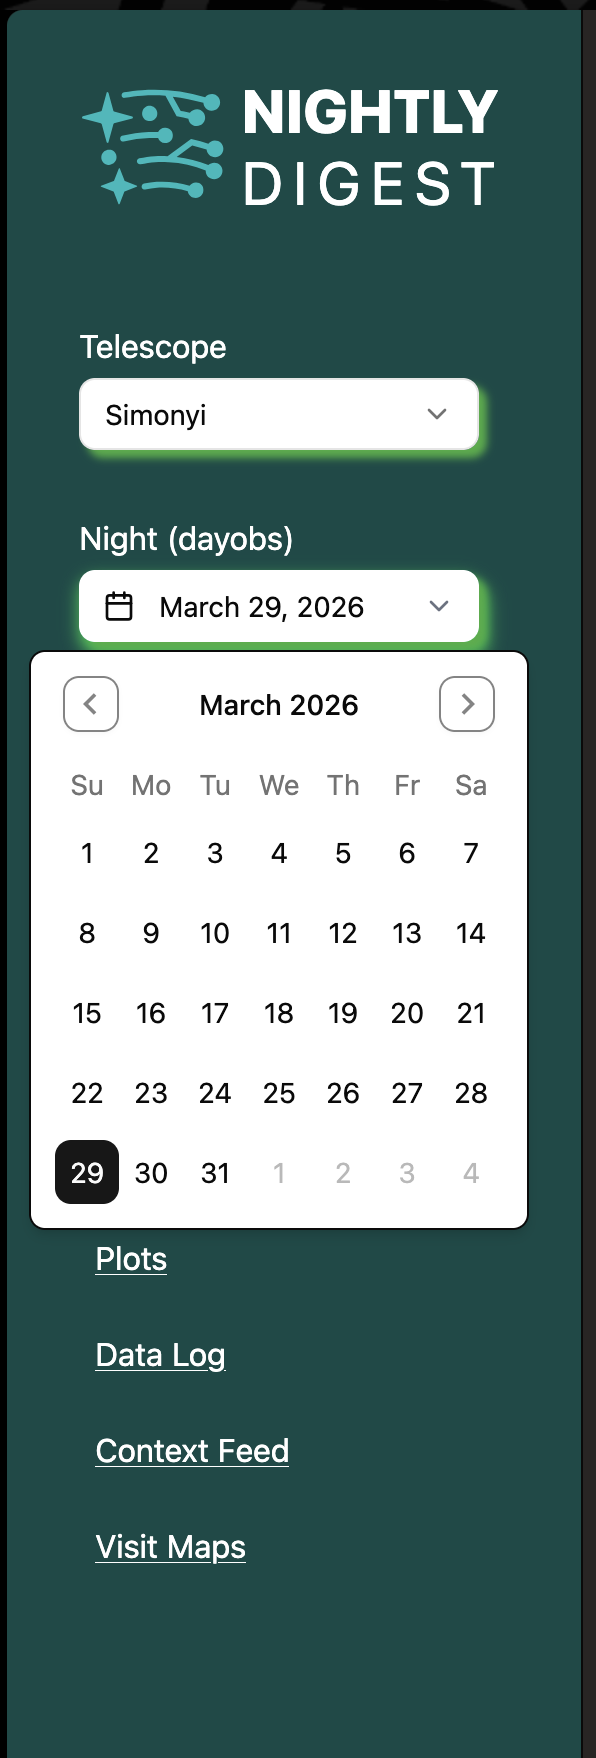
\includegraphics[height=10cm]{images/sidebar-calendar.png} &
    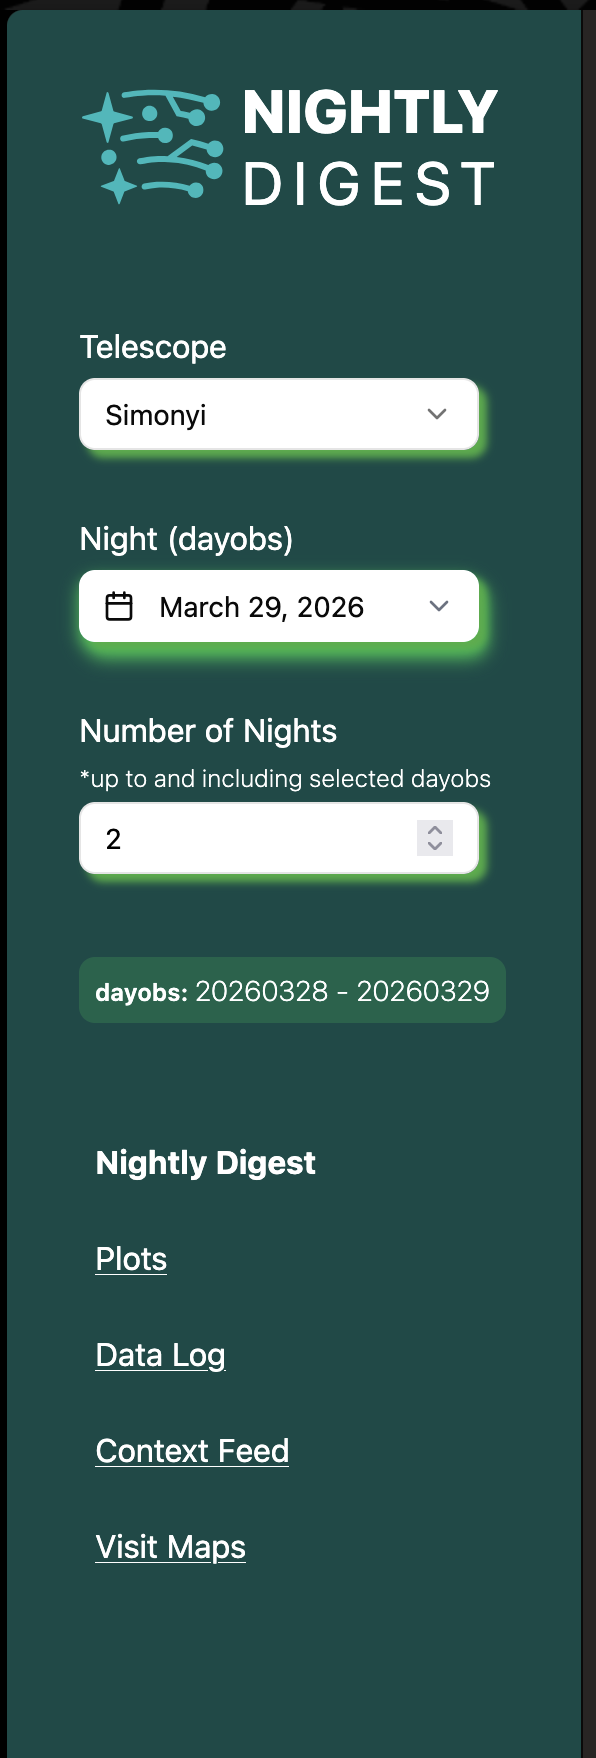
\includegraphics[height=10cm]{images/sidebar.png}
   \end{tabular}
   \end{center}
   \caption[example]
   { \label{fig:sidebar}
The Nightly Digest Sidebar contains selectable menus for telescope, night, and number
of nights. Below these parameters, the selected observation day is displayed.
Navigation to ~\ref{sec:addpages} is shown below.}
   \end{figure}

\FloatBarrier
   \subsection{The Nightly Digest page}

Across the top of the Nightly Digest [Fig ~\ref{fig:digest}], we display four summary
cards: Nighttime Exposures, Open Shutter Efficiency, Time Loss, and Jira Tickets.
The \textbf{Nighttime Exposures} card displays the number of exposures, queried from ConsDB, that were
taken on-sky, with the observatory dome open. This card also indicates the number of
expected exposures calculated from daily Feature Based Scheduler (FBS) simulations to
predict how many exposures could be taken each night \cite{Naghib19, RTN-016}.
\textbf{Open Shutter Efficiency} builds on the number of exposures taken to aggregate
total time exposing on-sky and compares this to the time available, subtracting out any
time impacted by weather. The \textbf{Time Loss} card collects the time loss reported from the
Narrative Log entries, and reports a total number of hours and distribution between
weather and technical faults.
The \textbf{Jira Tickets} card displays the number of tickets
created in the time frame the user has selected, and includes a note for the number of updated tickets.
When clicking on the Jira card, a dialog box opens displaying a table of
these tickets with notable attributes, including a summary, the current status, and a link
to the issue in the ticketing system.

When a larger observation day range is selected these cards accumulate data from each
observation day. The combination of these four cards at the top of our application gives a
quick overview of how the observing time went, answering questions about the volume of
data taken, the efficiency of the time spent, and if there were significant losses in time
and where to look to address those gaps.  The rest of the page is broken down into larger
displays of data, combining multiple data sources. The following sections describe each of
these applets in more detail and how they work together to give a comprehensive view of the observing night(s) selected.

\begin{figure} [ht]
   \begin{center}
   \begin{tabular}{c} %% tabular useful for creating an array of images
   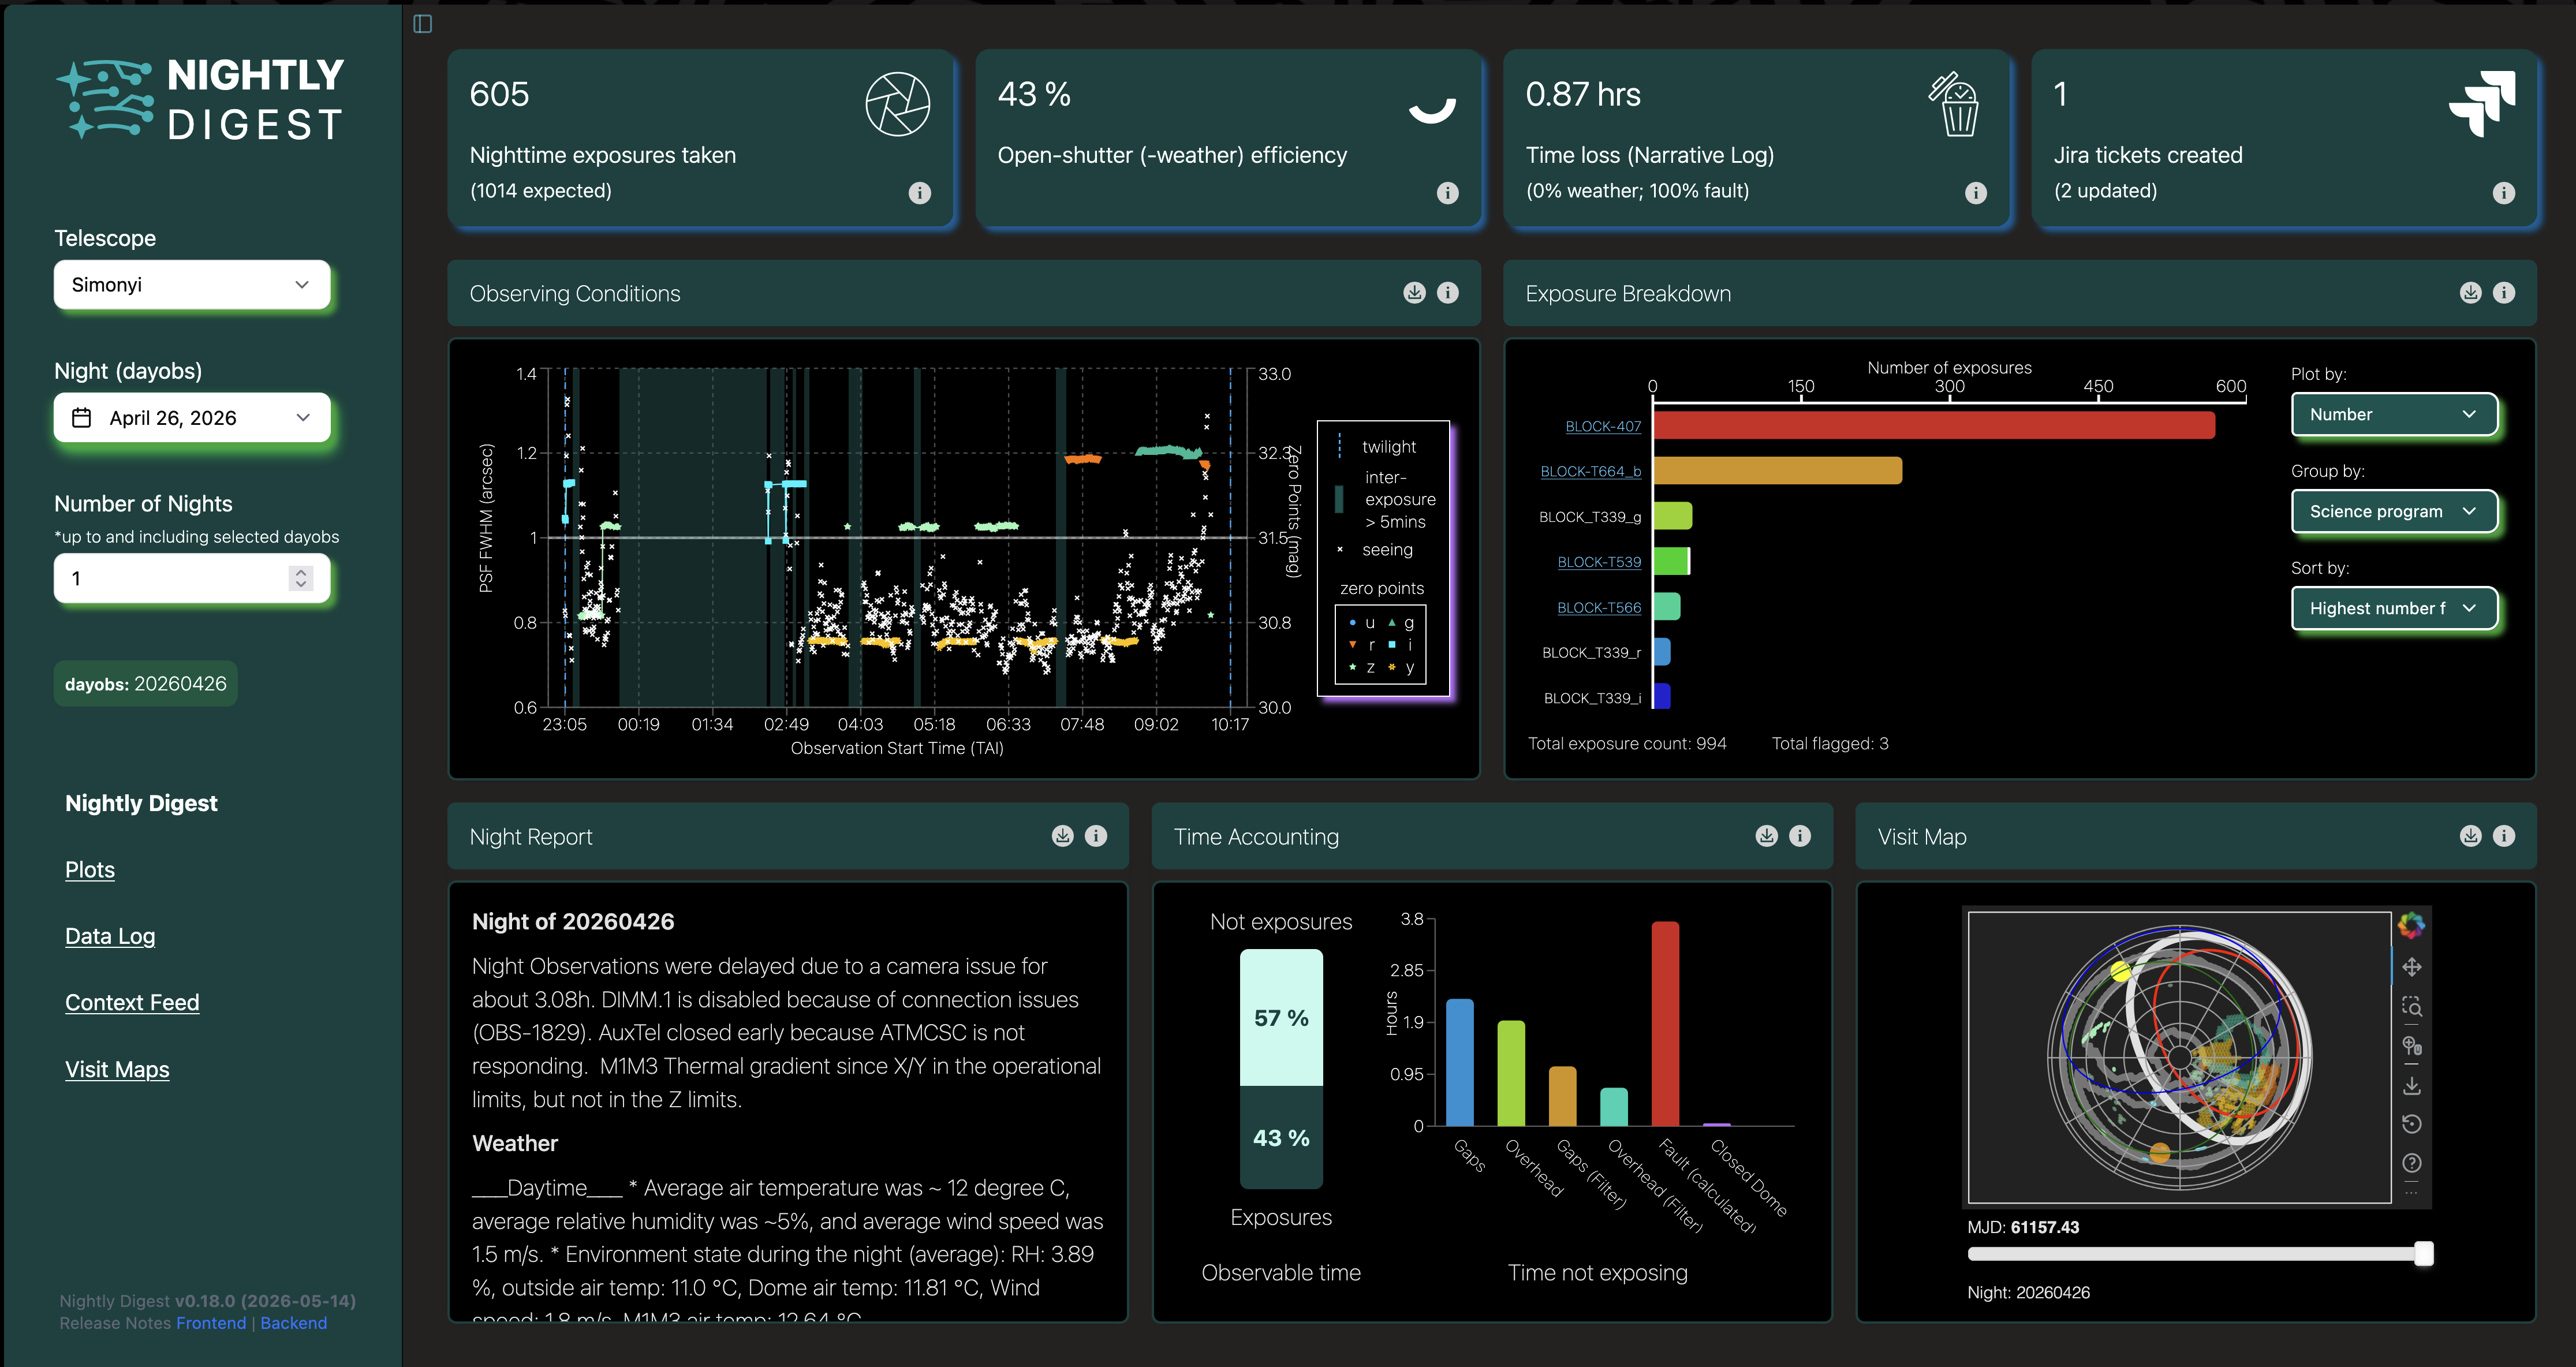
\includegraphics[height=9cm]{images/nightly-digest-full-page-better.png}
   \end{tabular}
   \end{center}
   \caption[example]
%>>>> use \label inside caption to get Fig. number with \ref{}
   { \label{fig:digest}
The Nightly Digest's main page displays multiple views of metrics both simple and more
complex. The applets and cards are arranged to display the data in a maximized browser
window but adjust to size and mobile displays.}
   \end{figure}

  \begin{figure} [ht]
   \begin{center}
   \begin{tabular}{c} %% tabular useful for creating an array of images
   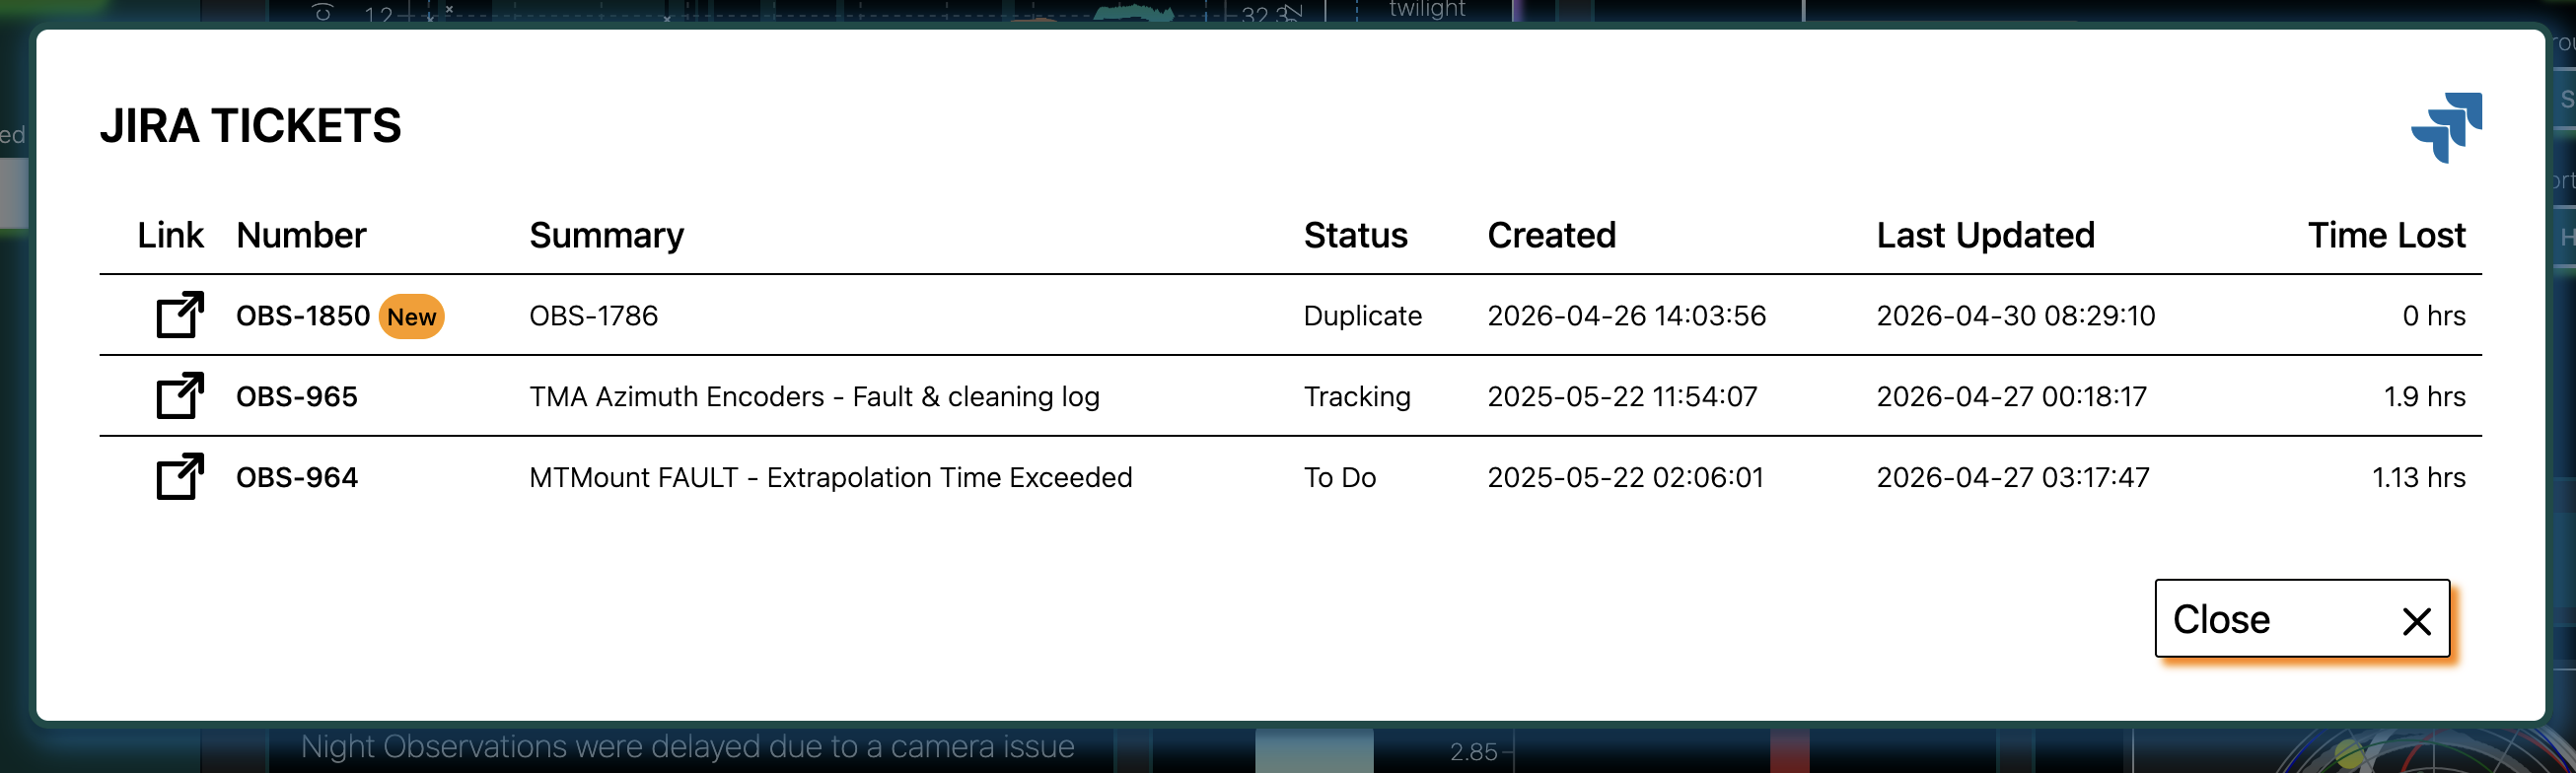
\includegraphics[height=5cm]{images/jira-tickets.png}
   \end{tabular}
   \end{center}
   \caption[example]
   { \label{fig:jira}
Click on the Jira ticket card to access a table displaying the specific tickets added and
their attributes. Click on a link to access our ticketing system.}
   \end{figure}


   \FloatBarrier
\subsubsection{Observing Conditions}

The Observing Conditions applet [Fig ~\ref{fig:observingconditions}] communicates the overall quality of the set of exposures
during the selected observation day range through a few different measures layered
together. Using exposure metadata from ConsDB and almanac information, this applet
displays a timeline of the exposures taken represented as their values of PSF FWHM and a
separate data point corresponding to the magnitude of their zero points categorized by
what filter was used for the exposure. This data interactively comes alive by mousing over
the filter legend as the plot displays only the data points from the filter the cursor
selects.

We are also able to see gaps in exposures highlighted in this chronological representation. The user can zoom
in on a selected portion of the plot to see a subset of data and hover over any of the data points to display
highlighted attributes for each exposure. This applet communicates the time distribution of exposures taken and
their measured qualities throughout the night. Users can infer observatory qualities from this combined
information including photometric depth and image quality. The interactivity
that we provide in this applet connects to both other applets on the page [Fig ~\ref{fig:obscondbreak}], and the zoom in selection holds when
navigating to other pages in the Nightly Digest for further investigation.

\begin{figure} [ht]
   \begin{center}
   \begin{tabular}{c} %% tabular useful for creating an array of images
   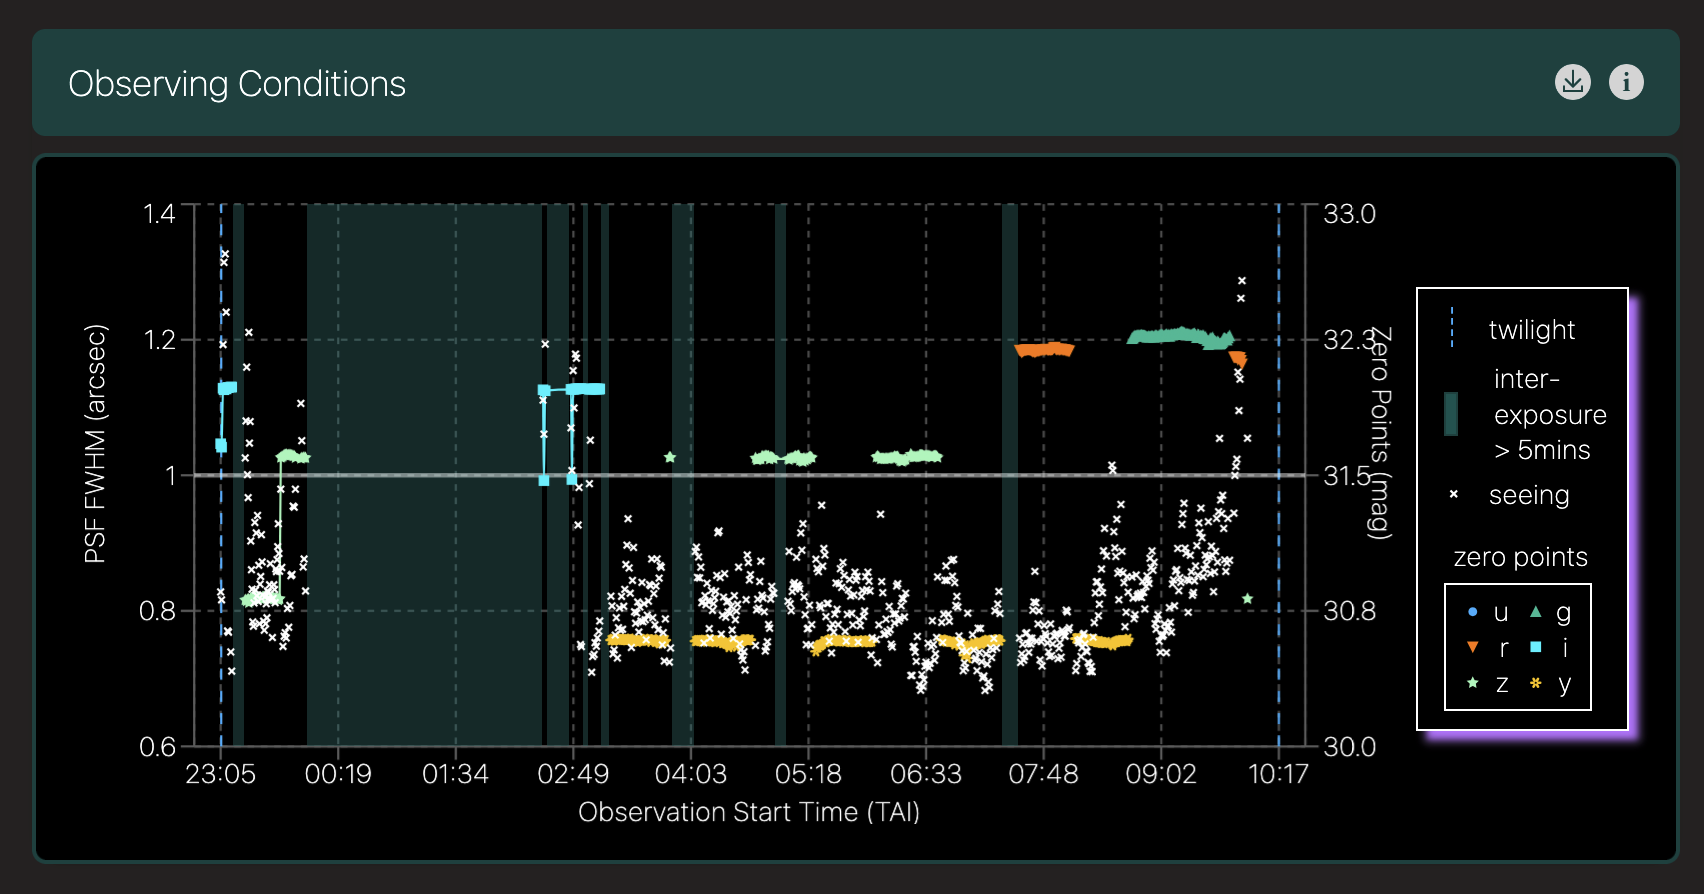
\includegraphics[height=8cm]{images/observing-conditions.png}
   \end{tabular}
   \end{center}
   \caption[example]
   { \label{fig:observingconditions}
The Observing Conditions applet displays the zero points and the point spread function
(PSF) for exposures taken during the selected time frame. The zero points are color-coded
based on which filter was active on the LSSTCam, and gaps between exposures are
highlighted in the background as dark green.}
   \end{figure}

  \begin{figure} [ht]
   \begin{center}
   \begin{tabular}{cc} %% tabular useful for creating an array of images
   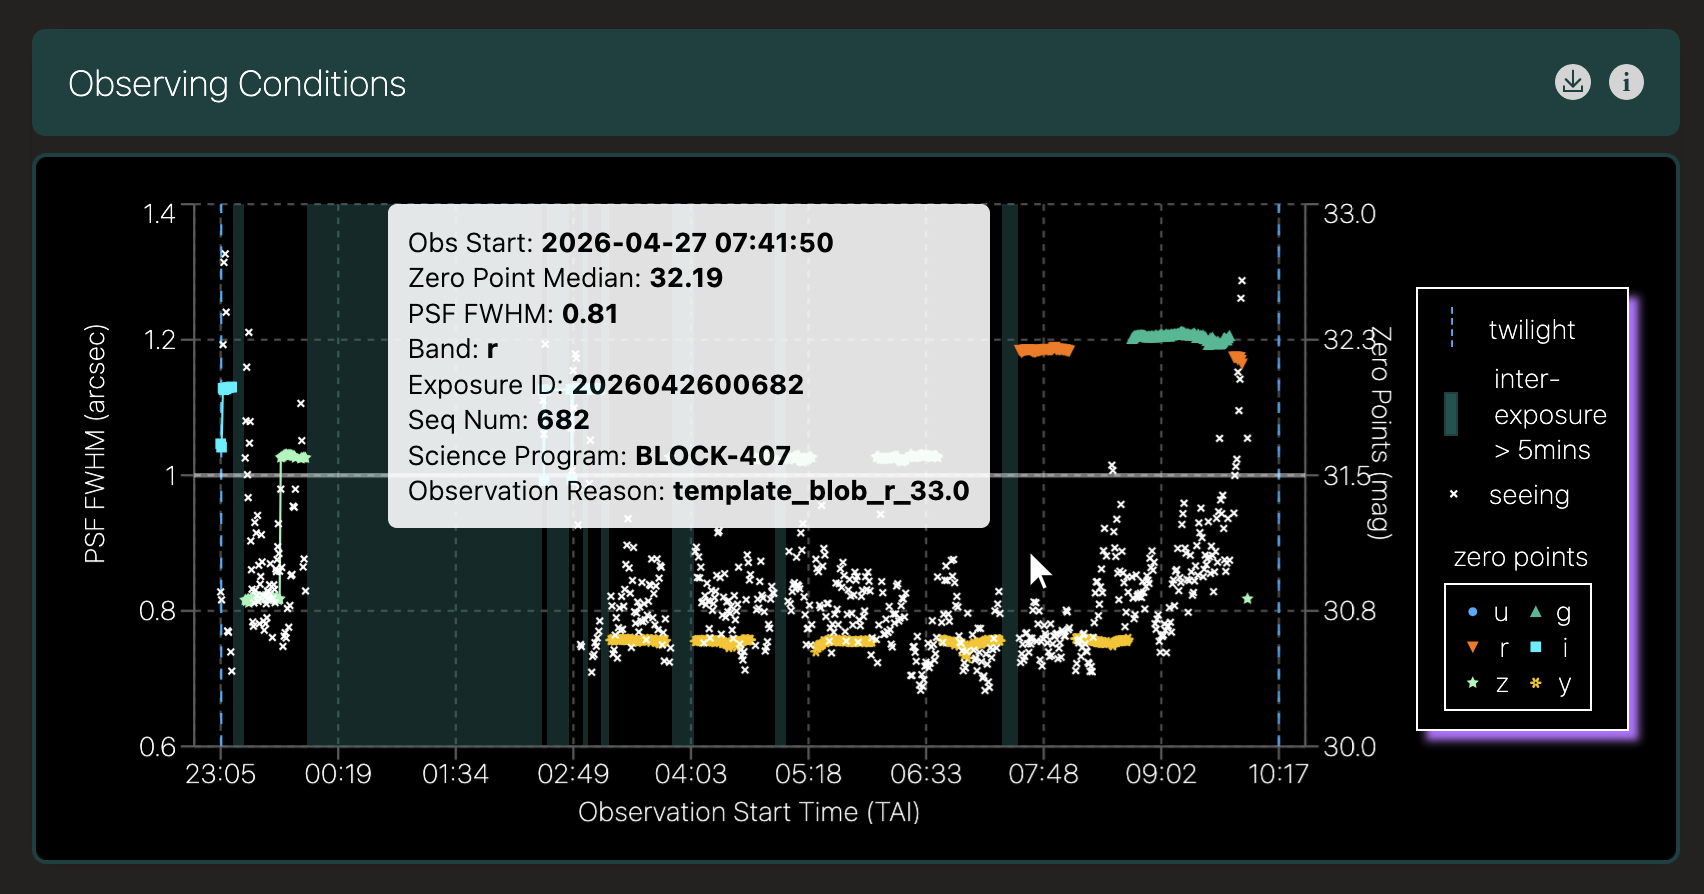
\includegraphics[height=4.2cm]{images/observing-conditions-focus.png} &
   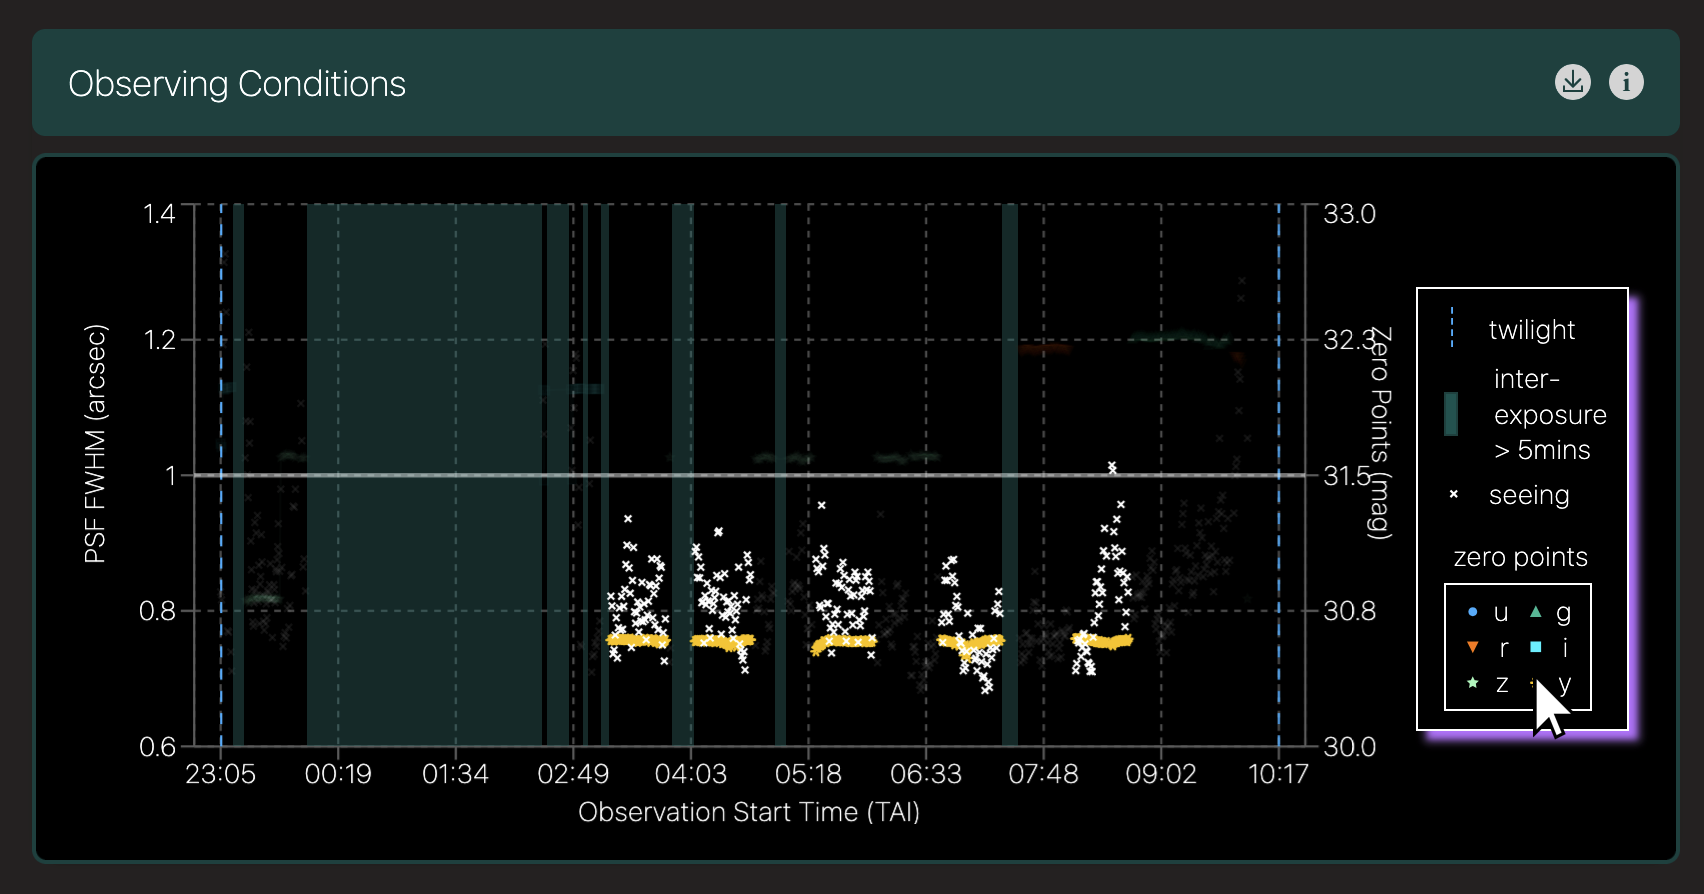
\includegraphics[height=4.2cm]{images/observing-conditions-filter.png}
   \end{tabular}
   \end{center}
   \caption[example]
   { \label{fig:obscondfocus}
Left: The Observing Conditions applet shows a dialog box when hovering over any individual data
point, displaying further attributes for any exposure. Right: Hover over a specific filter to the
bottom right of the observing conditions plot to see only that set of data displayed in the applet.}
   \end{figure}

   \FloatBarrier
\subsubsection{Exposure Breakdown}

The Exposure Breakdown applet [Fig ~\ref{fig:expbreakdown}] displays a horizontal bar chart that distributes the cumulative number
or time duration of exposures taken in any number of test case categories, observation reason,
target name, image type, or filter. This distribution can be sorted numerically or alphabetically.
If the user is interested in the exposures of a particular category, they can click on
that bar to navigate to a sorted Data Log page, filtering the exposure table to reveal
exactly how the night's visits spanned our science and engineering goals.

  \begin{figure} [ht]
   \begin{center}
   \begin{tabular}{c} %% tabular useful for creating an array of images
   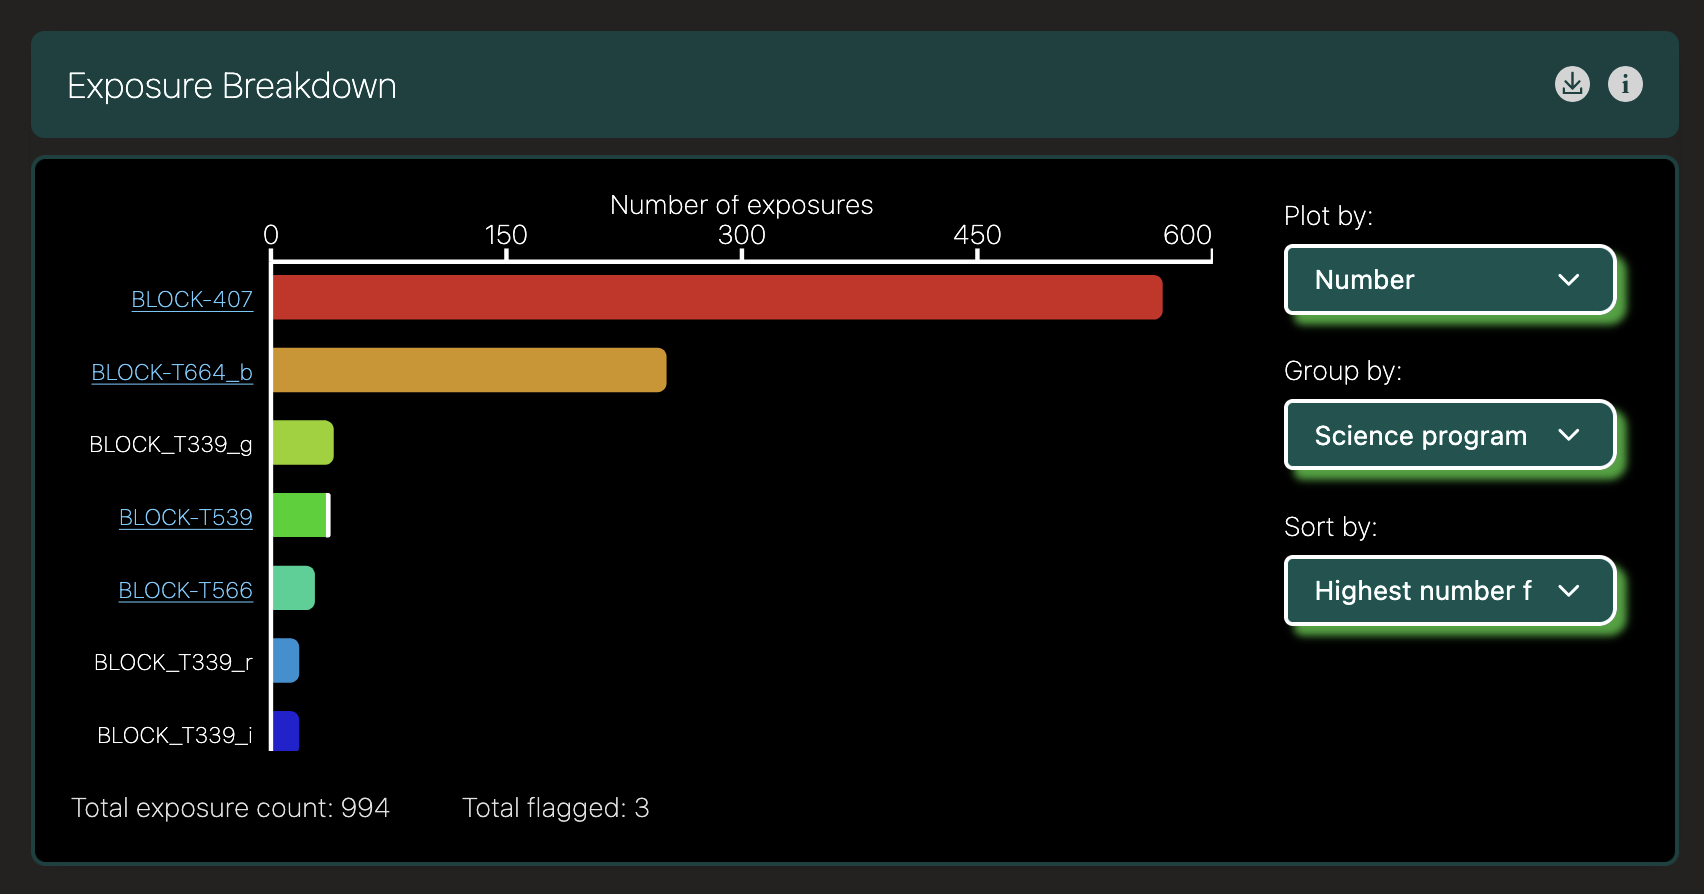
\includegraphics[height=8cm]{images/exposure-breakdown.png}
   \end{tabular}
   \end{center}
   \caption[example]
   { \label{fig:expbreakdown}
The Exposure Breakdown applet distributes the cumulative number or time duration of
exposures taken in any number of test case categories, observation reason, target name,
image type, or filter. This distribution can be sorted numerically or alphabetically.}
   \end{figure}


   \begin{figure} [ht]
   \begin{center}
   \begin{tabular}{c} %% tabular useful for creating an array of images
   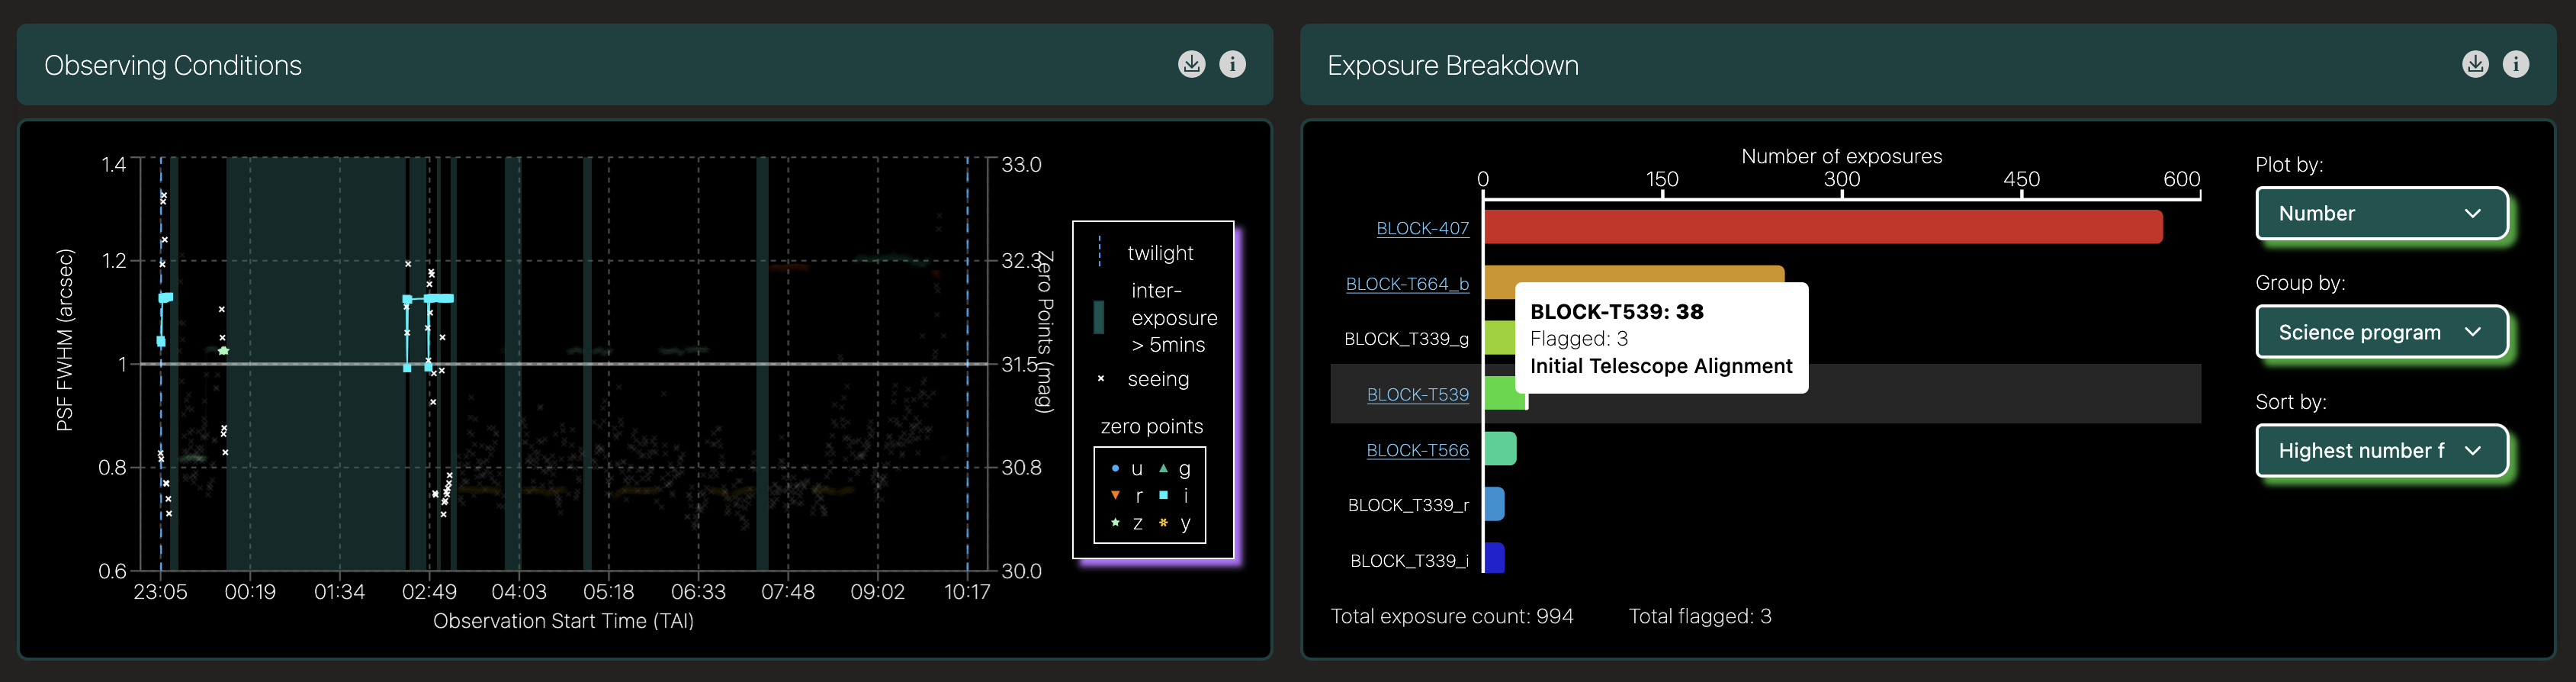
\includegraphics[height=4.5cm]{images/observing-conditions-breakdown.png}
   \end{tabular}
   \end{center}
   \caption[example]
   { \label{fig:obscondbreak}
The Observing Conditions applet and Exposure Breakdown applet work together through
interactivity. Highlight a category in Exposure Breakdown, and only the corresponding
exposures are displayed in Observing Conditions. }
   \end{figure}


   \FloatBarrier
\subsubsection{Night Report}

The Night Report applet [Fig ~\ref{fig:nightreport}] is the most narrative driven visual on the main page. This applet
queries data from the Night Log to represent the summary the Observing Specialists write
at the end of the observation day. The report contains a summary, weather conditions, a
detailed report, and a list of Observing Specialists and other staff who participated in
the summit operations directly, usually in person. When multiple days are selected, users
can navigate each observation day via a drop down menu, or scroll continuously through the
summaries. This high level summary of the events during each observation day is presented
to connect the numerical data presented elsewhere on the page and add context to which
tests were run, what anomalies were encountered, and give deeper understanding to how the
volume and quality of exposures ties to the way the available observing time was spent.

  \begin{figure} [ht]
   \begin{center}
   \begin{tabular}{c} %% tabular useful for creating an array of images
   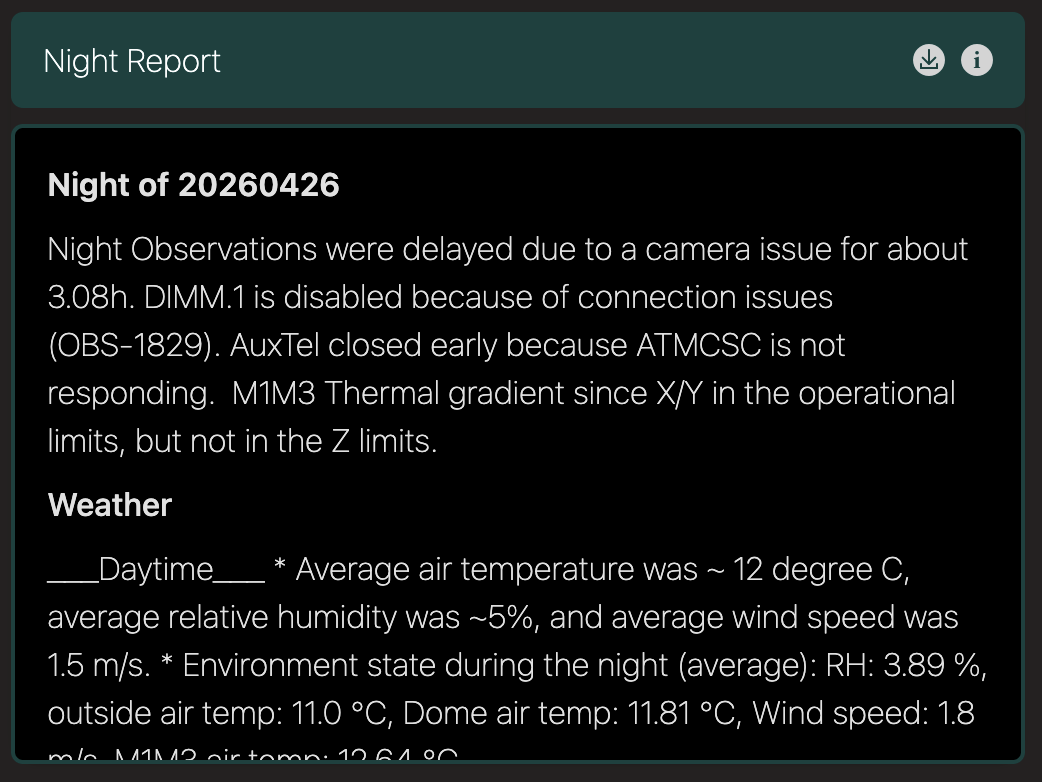
\includegraphics[height=8cm]{images/night-report.png}
   \end{tabular}
   \end{center}
   \caption[nightreport]
   { \label{fig:nightreport}
The end-of-the-night summary narrative is displayed in Night Report where sections include a summary,
weather conditions and scrolls when multiple observing days are selected.}
   \end{figure}

\subsubsection{Time Accounting}

The Time Accounting applet [Fig ~\ref{fig:timeacc}] is an evolving visualization to inform observatory metrics that
describe how the off-shutter time (when the camera is not actively exposing on the sky) is
used. It is critical to see how efficient the system is at taking observations, and to
enable different technical teams to dive into the time spent not observing.

The Nightly Digest's back end calculates how the available observing time was spent and
delineates between total exposure time and time not taking exposures. The ‘Not Exposures’
time is broken down into gaps between exposures, gaps and overhead related to filter
changes, calculated overhead time, calculated fault time, and time when the observatory
dome was closed during the night. We calculate fault time taking into account gaps,
overhead, total exposing time and comparing with total available observing time based on
almanac and weather information. These categories are either calculated internally or
gathered using the survey scheduling team’s software package \texttt{rubin\_nights} to
add slew and overhead detail to exposure data from ConsDB\cite{RTN-016}.
We also use time based data from the EFD including when the observatory dome opens and closes.

  \begin{figure} [ht]
   \begin{center}
   \begin{tabular}{c} %% tabular useful for creating an array of images
   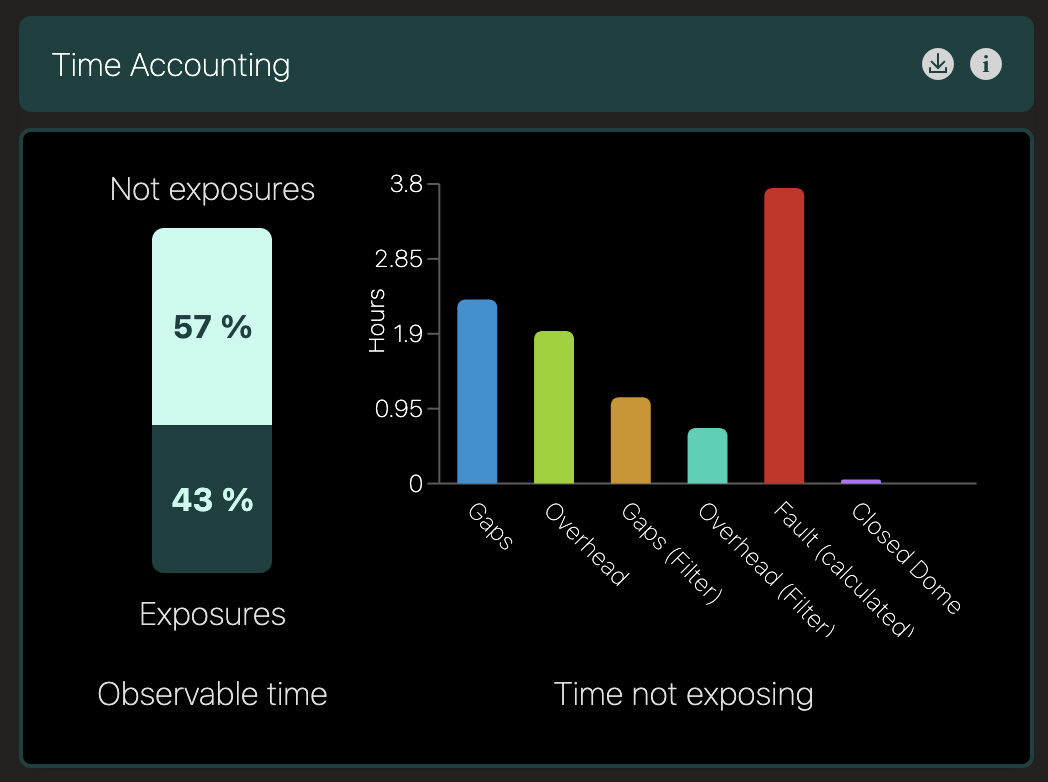
\includegraphics[height=8cm]{images/time-accounting.png}
   \end{tabular}
   \end{center}
   \caption[example]
   { \label{fig:timeacc}
The Time Accounting applet proportions the time spent during the night over the course of
the selected observation days between exposing time and not exposing. The Not Exposing
time is further broken down into gaps, overhead, fault, closed dome, and gaps/overhead
related to filter changes.}
   \end{figure}

The applets previously described cover observatory activities throughout the observation
period, and this applet adds further context about the time not represented in the volume
of exposures taken.

Our current iteration of the Time Accounting applet will soon be replaced to represent
further automated systems and information about observatory status as a whole, calculated
outside of the Nightly Digest [Fig ~\ref{fig:obsstatus}].

\begin{figure} [ht]
   \begin{center}
   \begin{tabular}{c} %% tabular useful for creating an array of images
   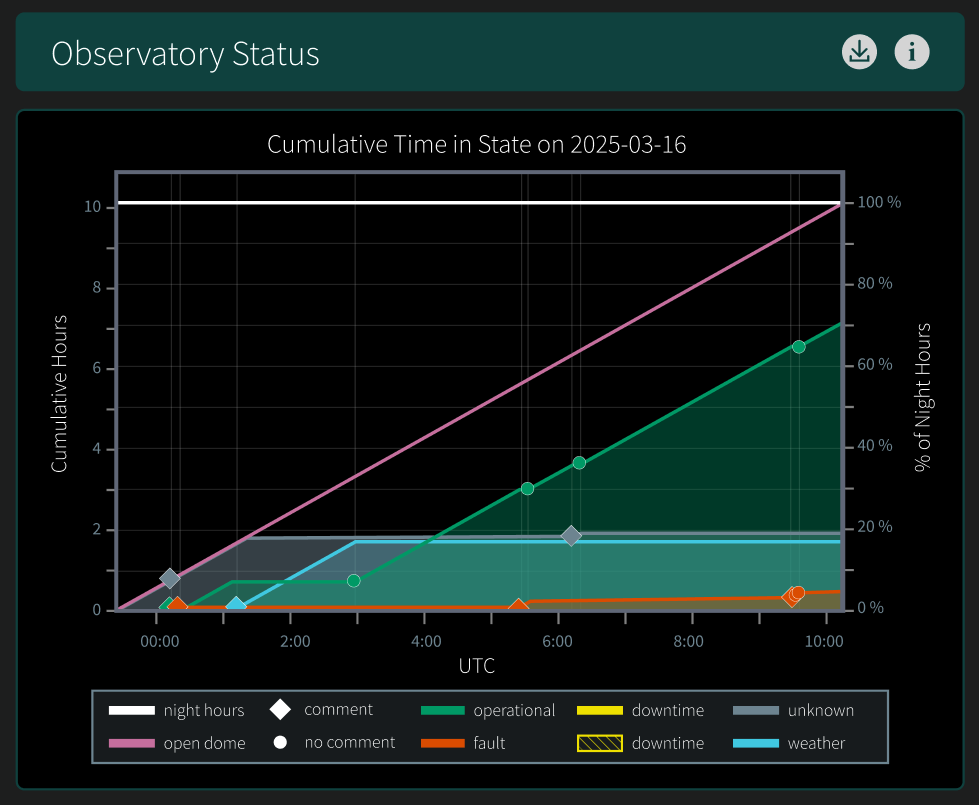
\includegraphics[height=8cm]{images/observatory-status.png}
   \end{tabular}
   \end{center}
   \caption[obsstatus]
   { \label{fig:obsstatus}
Mock up of Time Accounting/Observatory Status. Rubin Observatory is improving how we track
the state of the observatory, and we are updating our visualizations to reflect new automated Observatory States.
Here we see a model of the cumulative time in various states and when the states change throughout the observation night.
}
\end{figure}


\FloatBarrier
\subsubsection{Visit Map}

The Visit Map applet [Fig ~\ref{fig:vma}] shows an interactive planispheric projection of a full observation
day’s visits\footnote[1]{We use ‘visit’ and ‘exposure’ to refer to the same piece of data.
Rubin Observatory once considered multiple shorter exposures to compose one visit, but
currently they share a one to one relationship.}. We get this RA and Dec data from ConsDB
for each exposure. This data is augmented with almanac data to display environmental
information relative to visit locations. The user can scroll this display over many nights
adjacent to the currently selected observation day or range to see the pattern of where
the observatory is exposing on the sky. This applet communicates what type of activities
the summit is performing, engineering tests could look quite different than LSST-like
observations, while survey-like activities will sweep across an area filling it in. The
Visit Map is highly detailed, including markers for the moon, sun, ecliptic, plane of the
milky way and other labels. From this applet, users learn if their area of interest was
exposed, and they can understand further context including how the exposures shown in
other applets was distributed across the sky for that period. This data visualization is
expanded upon in a Visit Map page~\ref{sec:vmp} and is a result of our inspiration from and
collaboration with the survey scheduling team who has been a great help in our development
and integration of this plot \cite{RTN-016}.

  \begin{figure} [ht]
   \begin{center}
   \begin{tabular}{c} %% tabular useful for creating an array of images
   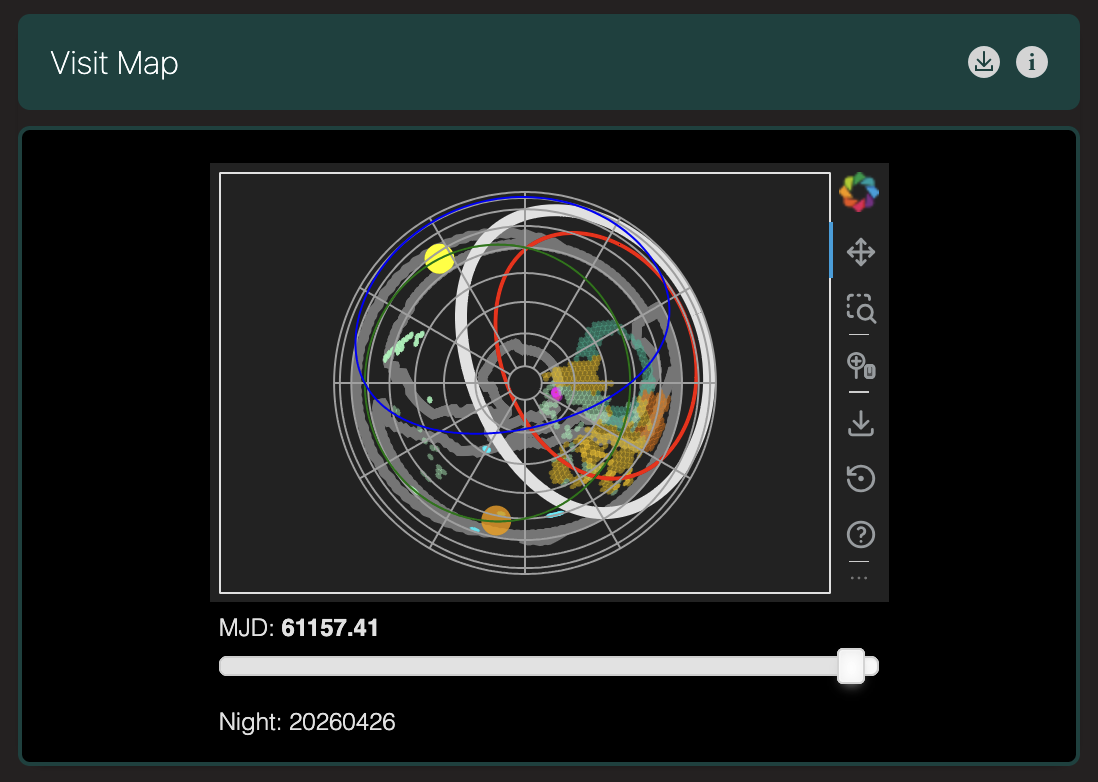
\includegraphics[height=8cm]{images/visit-map-applet.png}
   \end{tabular}
   \end{center}
   \caption[visitmap]
   { \label{fig:vma}
The Visit Map applet displays a planispheric projection of the visits taken within an
observation day selected and includes the sun, moon, ecliptic, and horizon locations. This
applet is interactive as one can scroll through time.}
   \end{figure}

\FloatBarrier
\section{Supporting Pages}
\label{sec:addpages}

While the Nightly Digest’s main summary page [Fig ~\ref{fig:digest}] was our initial focus, we have found that
additional pages support our use cases of debugging and adding context. These pages tie
into our core questions~\ref{sec:corequestions} and expand upon our summary page applets while adding complexity
and depth to the information provided.

One theme of logging that continues through each of these pages is our shared
chronological understanding of data. This is represented in three of the four additional
pages via a timeline UI component, and in the fourth as a slider through time. Initially
in the Context Feed page [Fig ~\ref{fig:cftimeline}], our timeline component [Fig ~\ref{fig:timeline}]
displays a horizontal area marking events as vertical lines from left to right. Each of our timelines
has a pink selection area so users may modify the time selected and displayed in the data pages to span multiple
observation days, partial selections across multiple days [Fig ~\ref{fig:timelinemulti}],
to even a single exposure or event.

  \begin{figure} [ht]
   \begin{center}
   \begin{tabular}{c} %% tabular useful for creating an array of images
   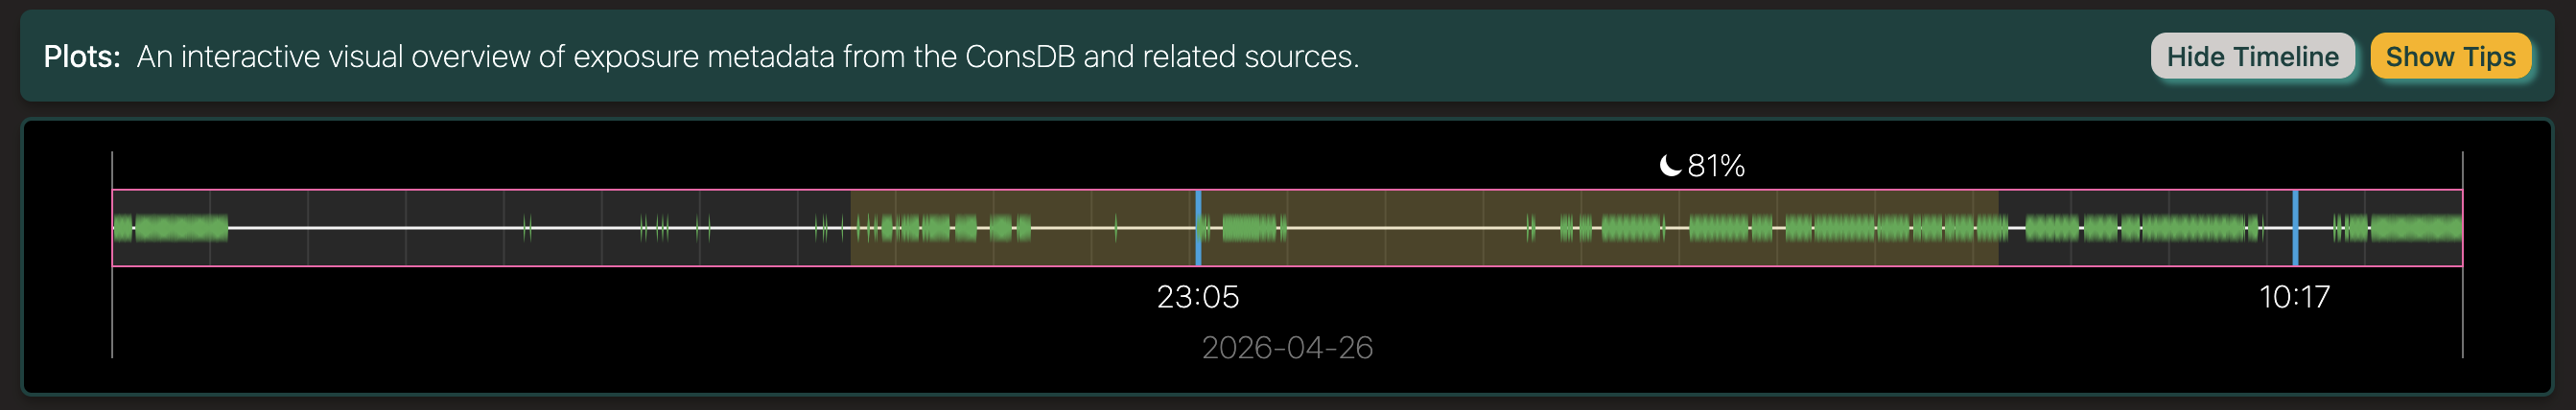
\includegraphics[height=2.75cm]{images/timeline-plots-single-short.png}
   \end{tabular}
   \end{center}
   \caption[timeline]
   { \label{fig:timeline}
The timelines in the Nightly Digest allow the user to select a portion of data to view in
tables or data in the corresponding page. This allows the user to focus in on only their
time frame of interest. }
   \end{figure}

  \begin{figure} [ht]
   \begin{center}
   \begin{tabular}{c} %% tabular useful for creating an array of images
   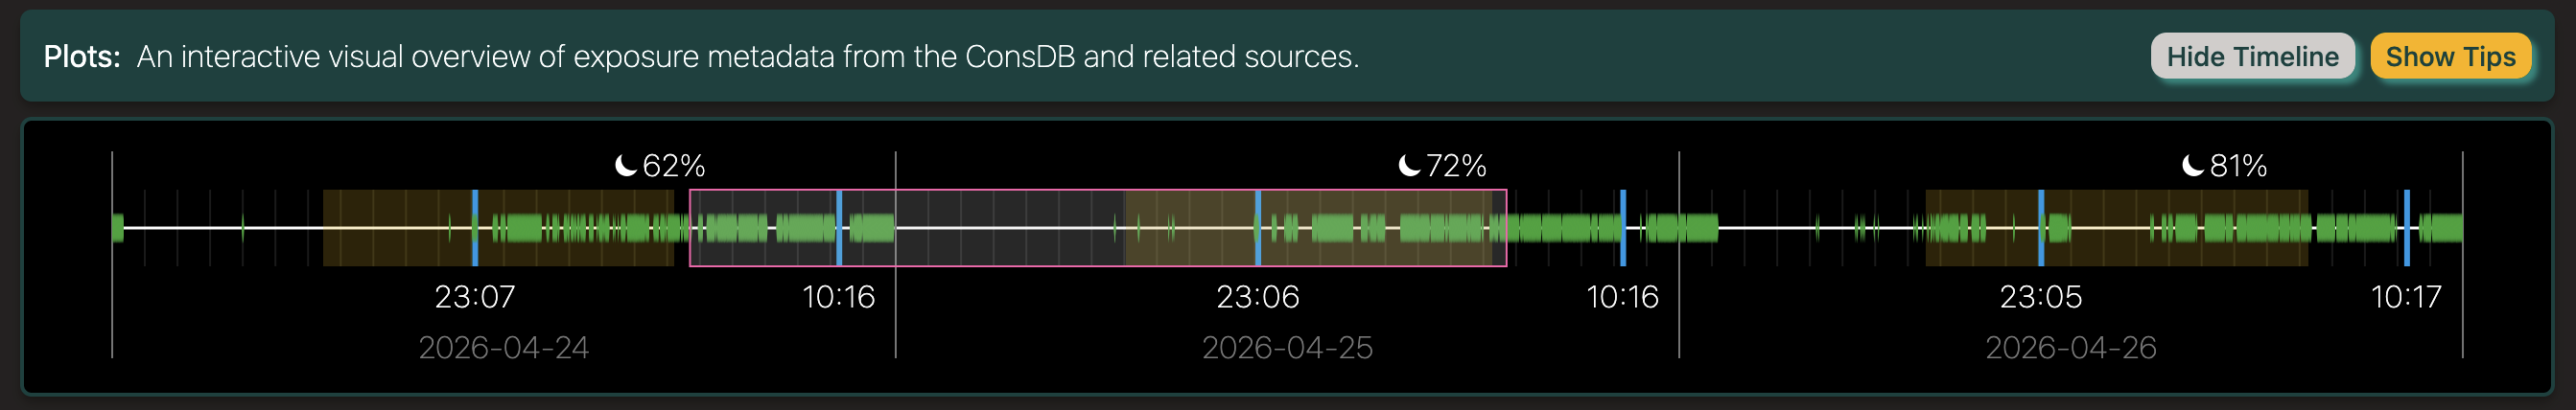
\includegraphics[height=2.75cm]{images/timeline-plots-multi-short.png}
   \end{tabular}
   \end{center}
   \caption[timelinemulti]
   { \label{fig:timelinemulti}
Multiple observation days can be selected in the Nightly Digest where the timelines update
to include this greater time period of data. The user can select portions of multiple
nights together as shown here. }
   \end{figure}

  \begin{figure} [ht]
   \begin{center}
   \begin{tabular}{c} %% tabular useful for creating an array of images
   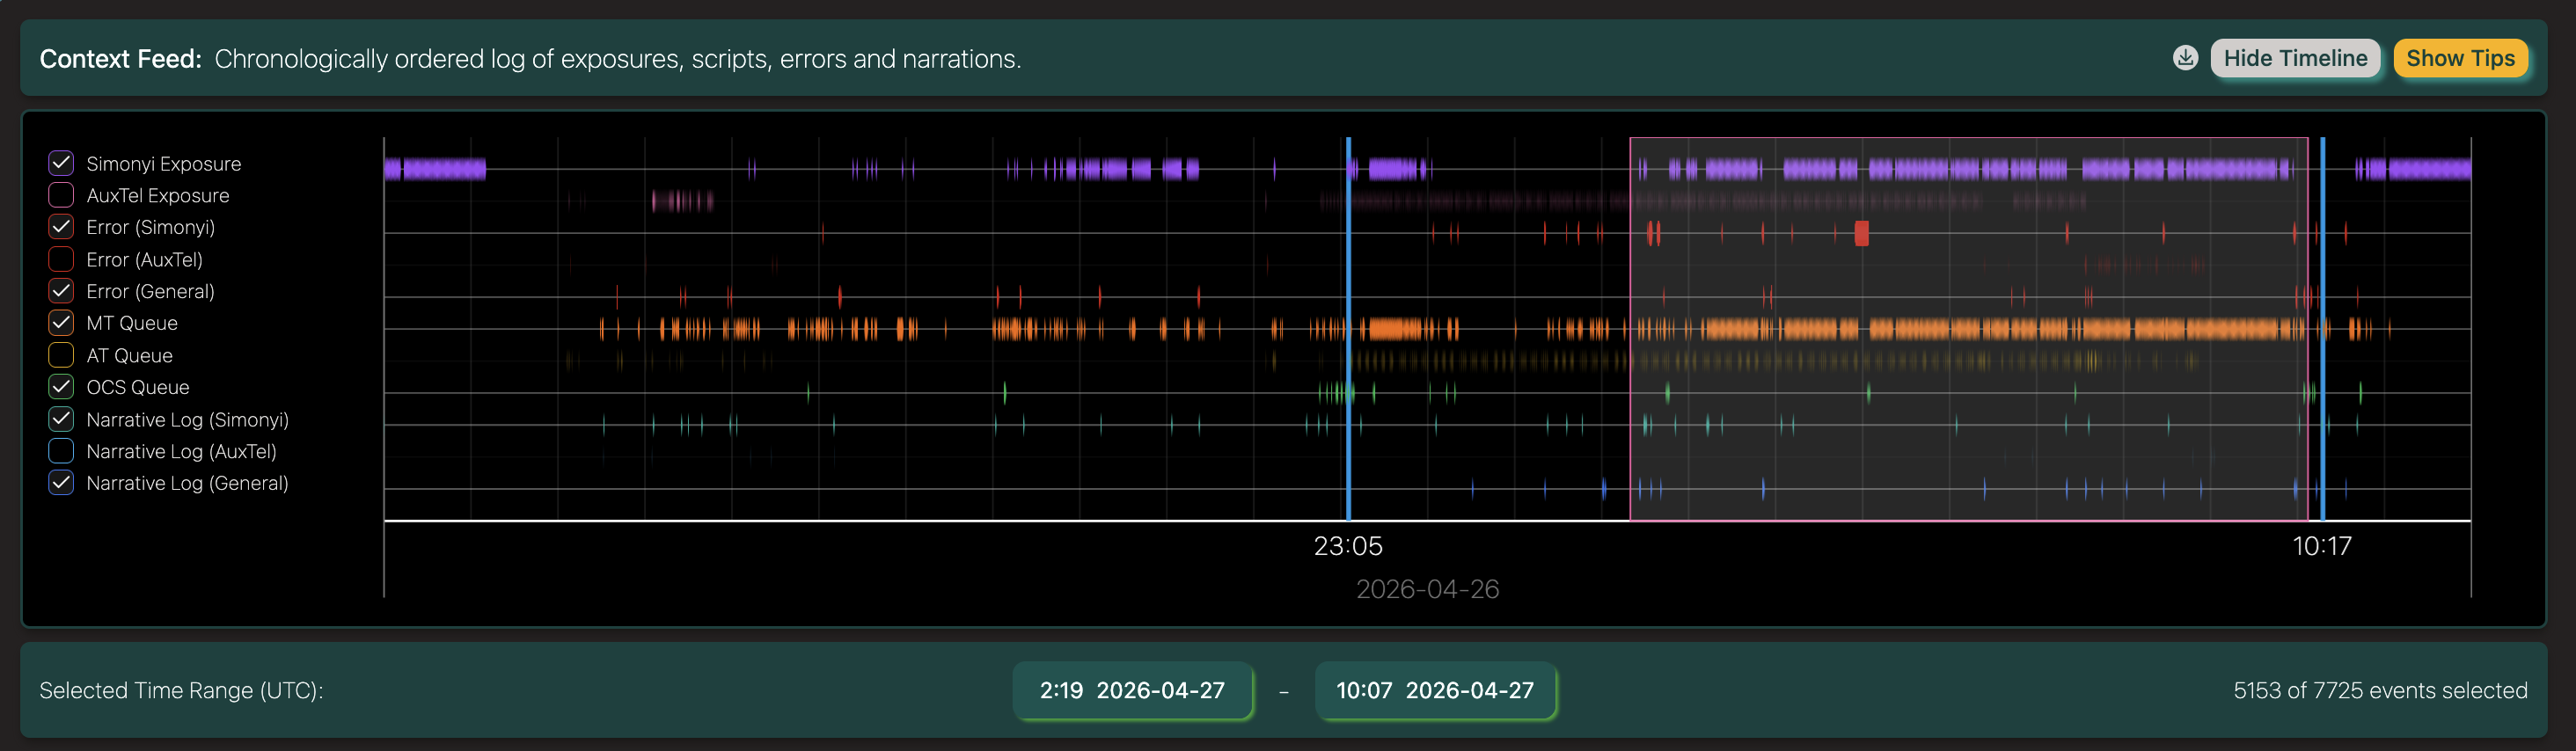
\includegraphics[height=5cm]{images/context-feed-timeline.png}
   \end{tabular}
   \end{center}
   \caption[example]
   { \label{fig:cftimeline}
The timeline in the Context Feed page displays each category of telemetric and narrative
log message in relationship to the time frame selected. These categories include
exposures, script errors, and observer narrative messages.}
   \end{figure}

   \FloatBarrier
\subsection{Plots}

The Plots page [Fig ~\ref{fig:plots}] expands on the Observing Conditions applet [Fig ~\ref{fig:observingconditions}]
to satisfy the users’ desires to easily access exposure metadata and trends across the
selected observation day range. This page displays numerous pre-created plots from
many exposure attributes in ConsDB, and by default displays airmass, PSF FWHM, photometric zero points, and sky brightness.
The user may also select a portion of any plot to zoom in on, and the additional plots
displayed synchronously adjust to that new time period. For more complex plotting and data exploration,
users are encouraged to use a jupyter notebook in the RSP
where they can query the same data sources and create custom plots with more freedom and flexibility.

  \begin{figure} [ht]
   \begin{center}
   \begin{tabular}{c} %% tabular useful for creating an array of images
   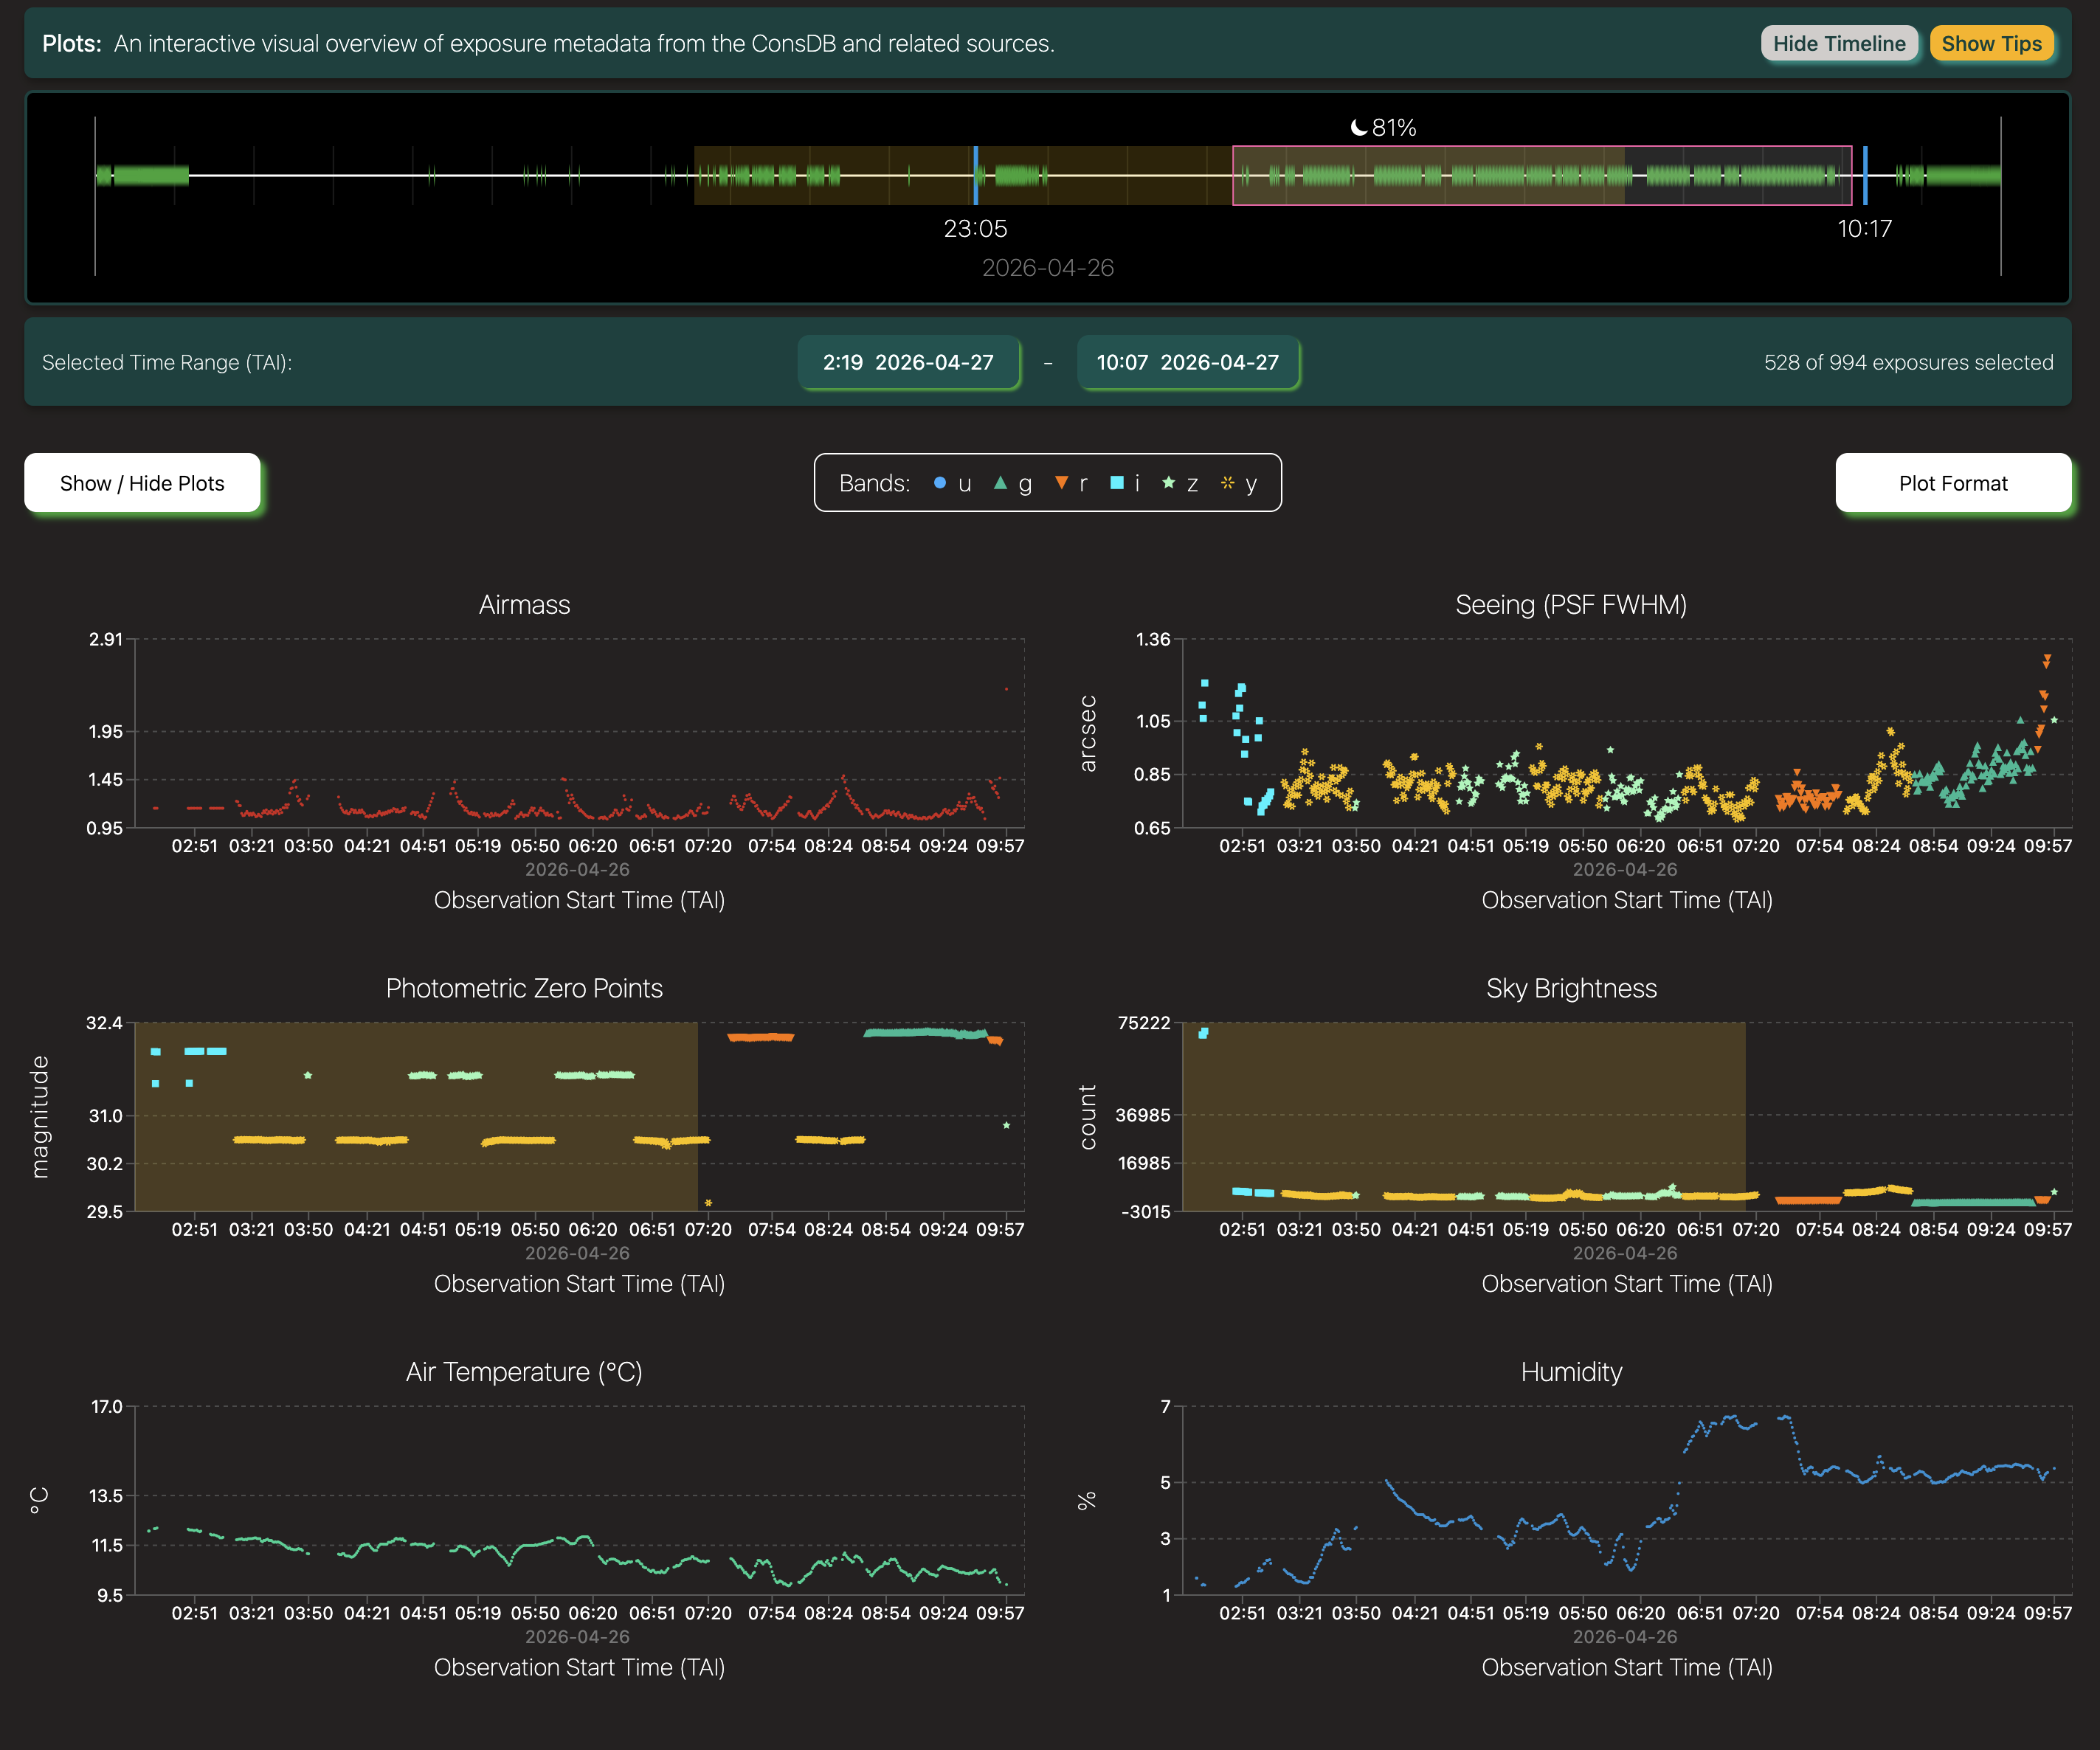
\includegraphics[height=13cm]{images/plots-page.png}
   \end{tabular}
   \end{center}
   \caption[example]
   { \label{fig:plots}
The Plots page displays a configurable set of data during the selected time frame
corresponding to the timeline at the top of the page. Each plot displays data based on the
attributes and metadata provided from ConsDB.}
   \end{figure}

\FloatBarrier
\subsection{Data Log}

The Data Log page [Fig ~\ref{fig:datalog}] expands on the main summary page’s 
Exposure Breakdown applet [Fig ~\ref{fig:expbreakdown}]
by providing a table of all exposures within the selected observation day range. The columns
display exposure metadata from ConsDB and comments from the Exposure Log associated with
each exposure. This table is scrollable and the visible columns can be selected [Fig ~\ref{fig:datalogcols}]
and defined by the user. Any column may also be sorted or grouped by the available values [Fig ~\ref{fig:dataloggroup}] for
each attribute, allowing users to categorize data to understand groupings of exposures
according to their area of focus.

  \begin{figure} [ht]
   \begin{center}
   \begin{tabular}{c} %% tabular useful for creating an array of images
   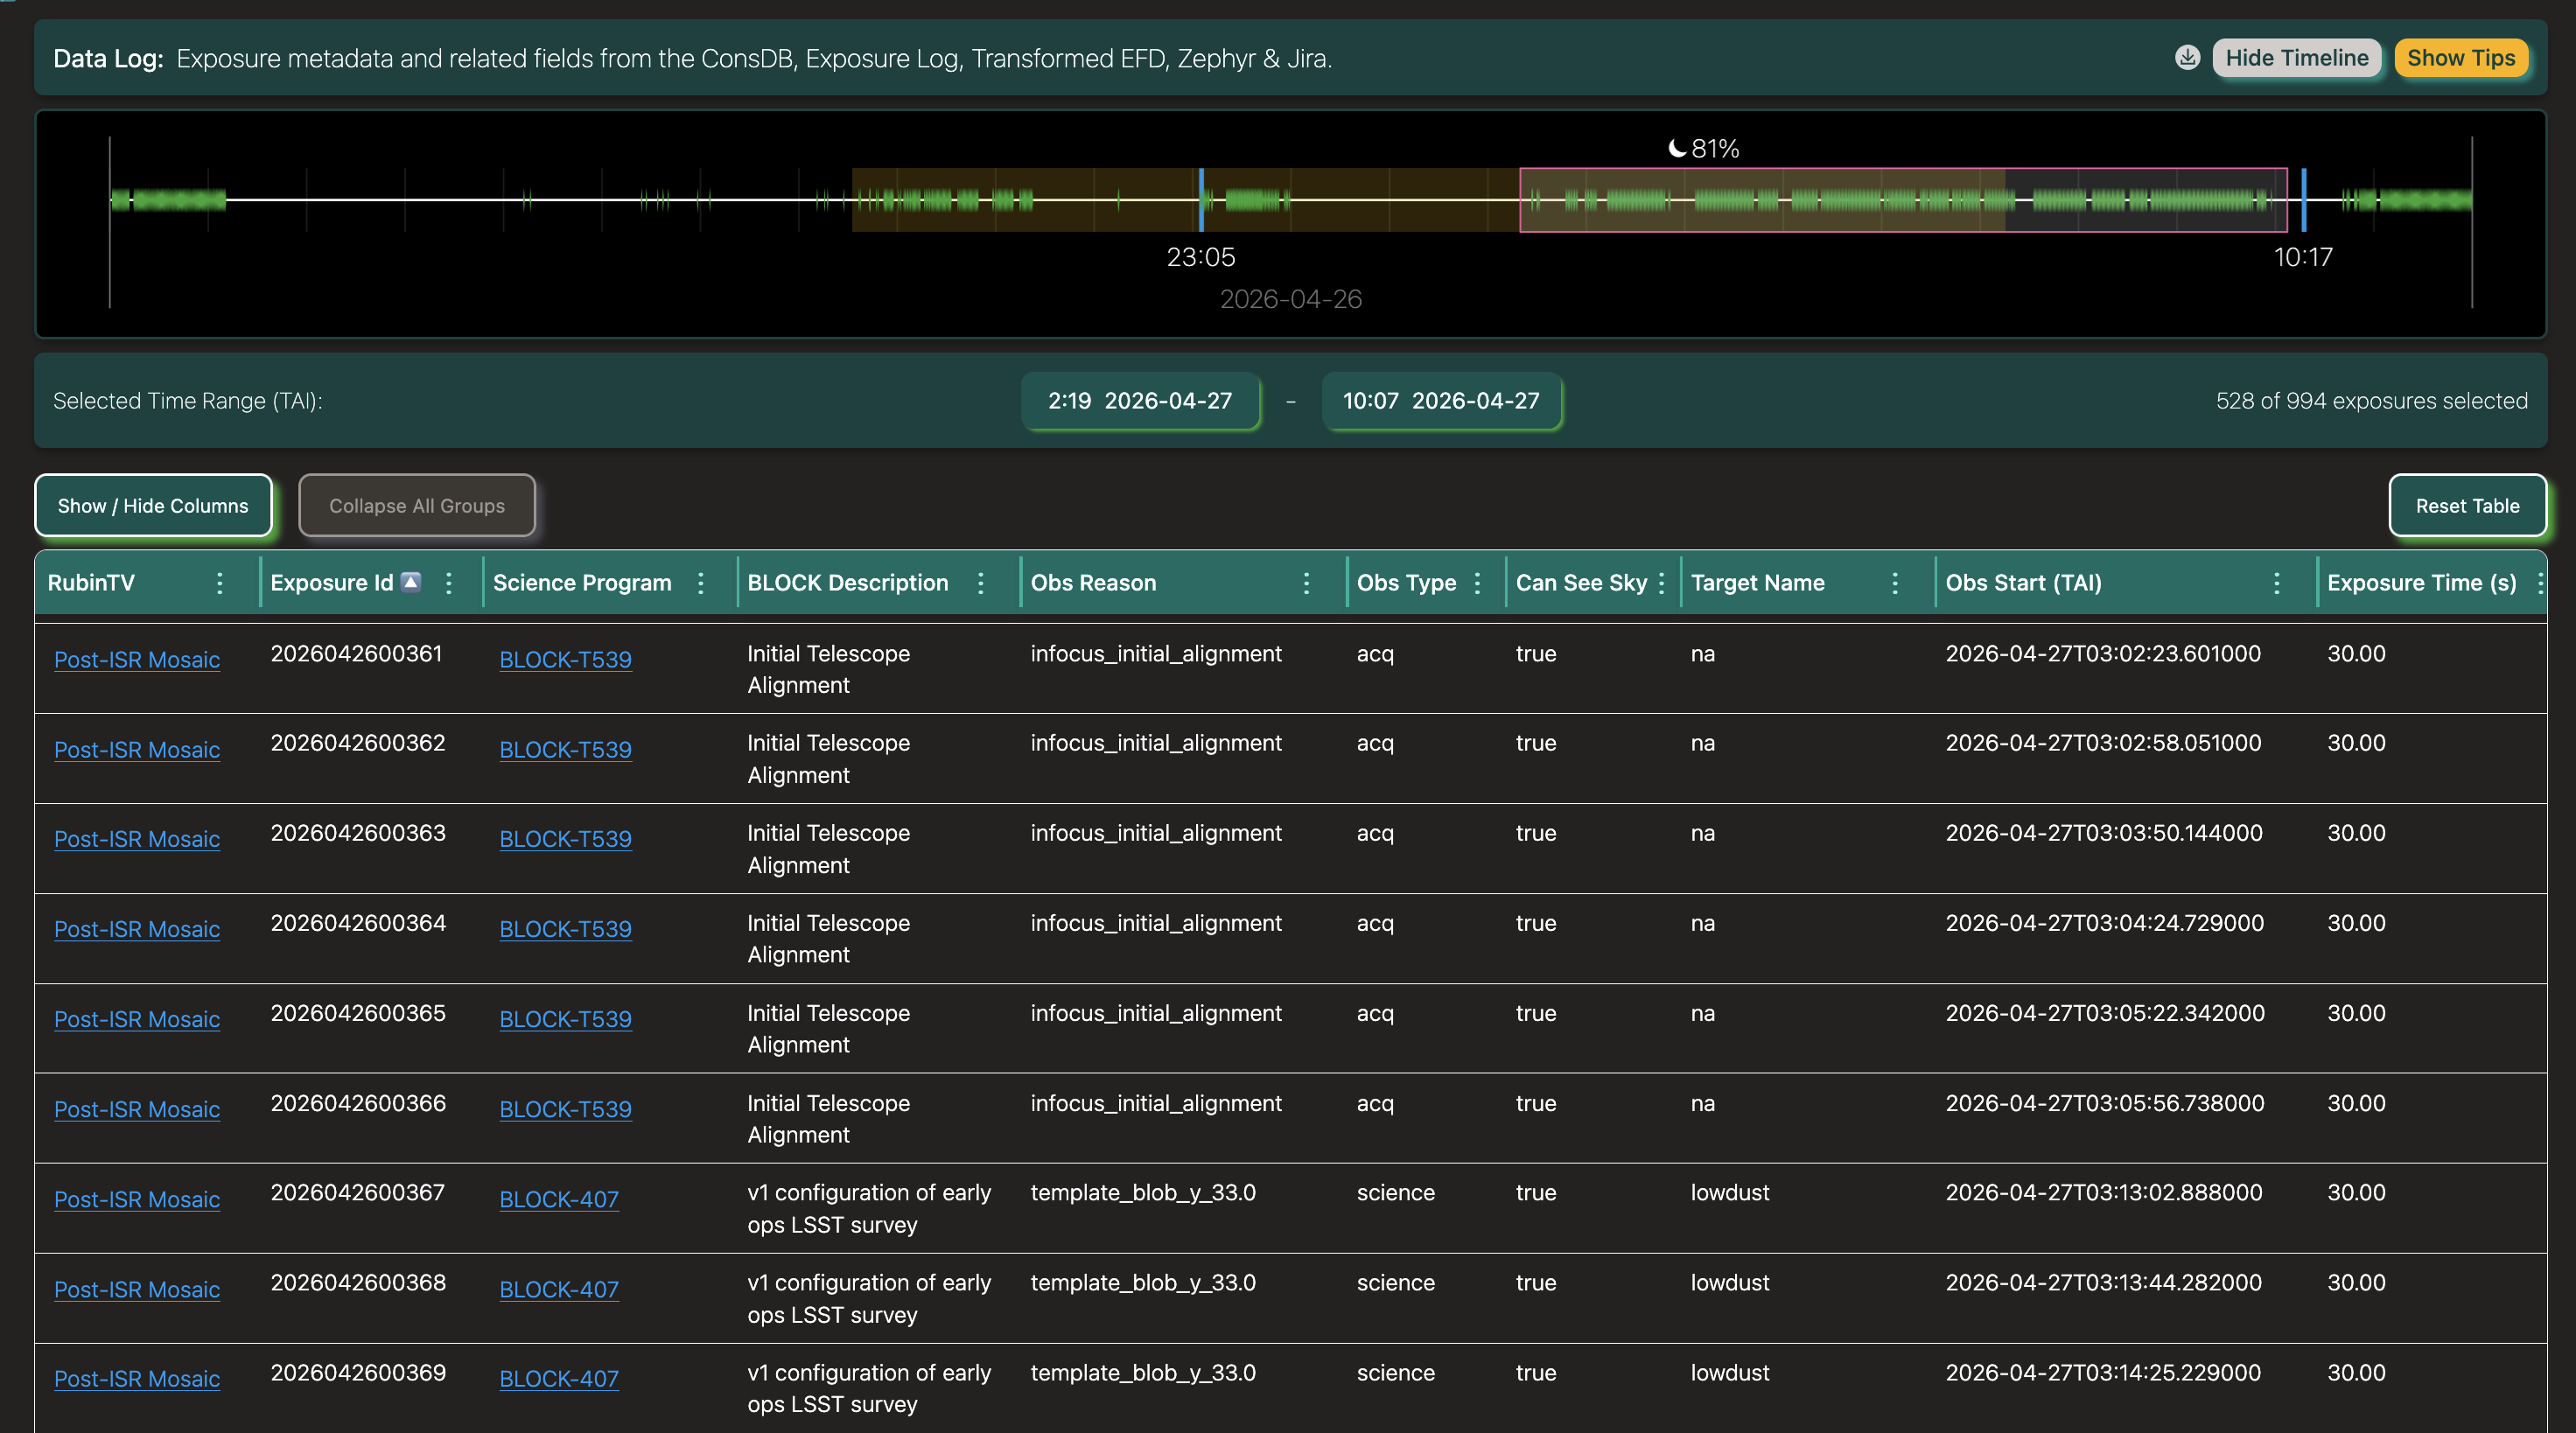
\includegraphics[height=8cm]{images/data-log-short.png}
   \end{tabular}
   \end{center}
   \caption[example]
   { \label{fig:datalog}
The Data Log page includes a timeline of the exposures and when they were taken over the
time frame selected, or entire observation day, and displays this selected range of data
below in an interactive table.}
   \end{figure}

  \begin{figure} [ht]
   \begin{center}
   \begin{tabular}{c} %% tabular useful for creating an array of images
   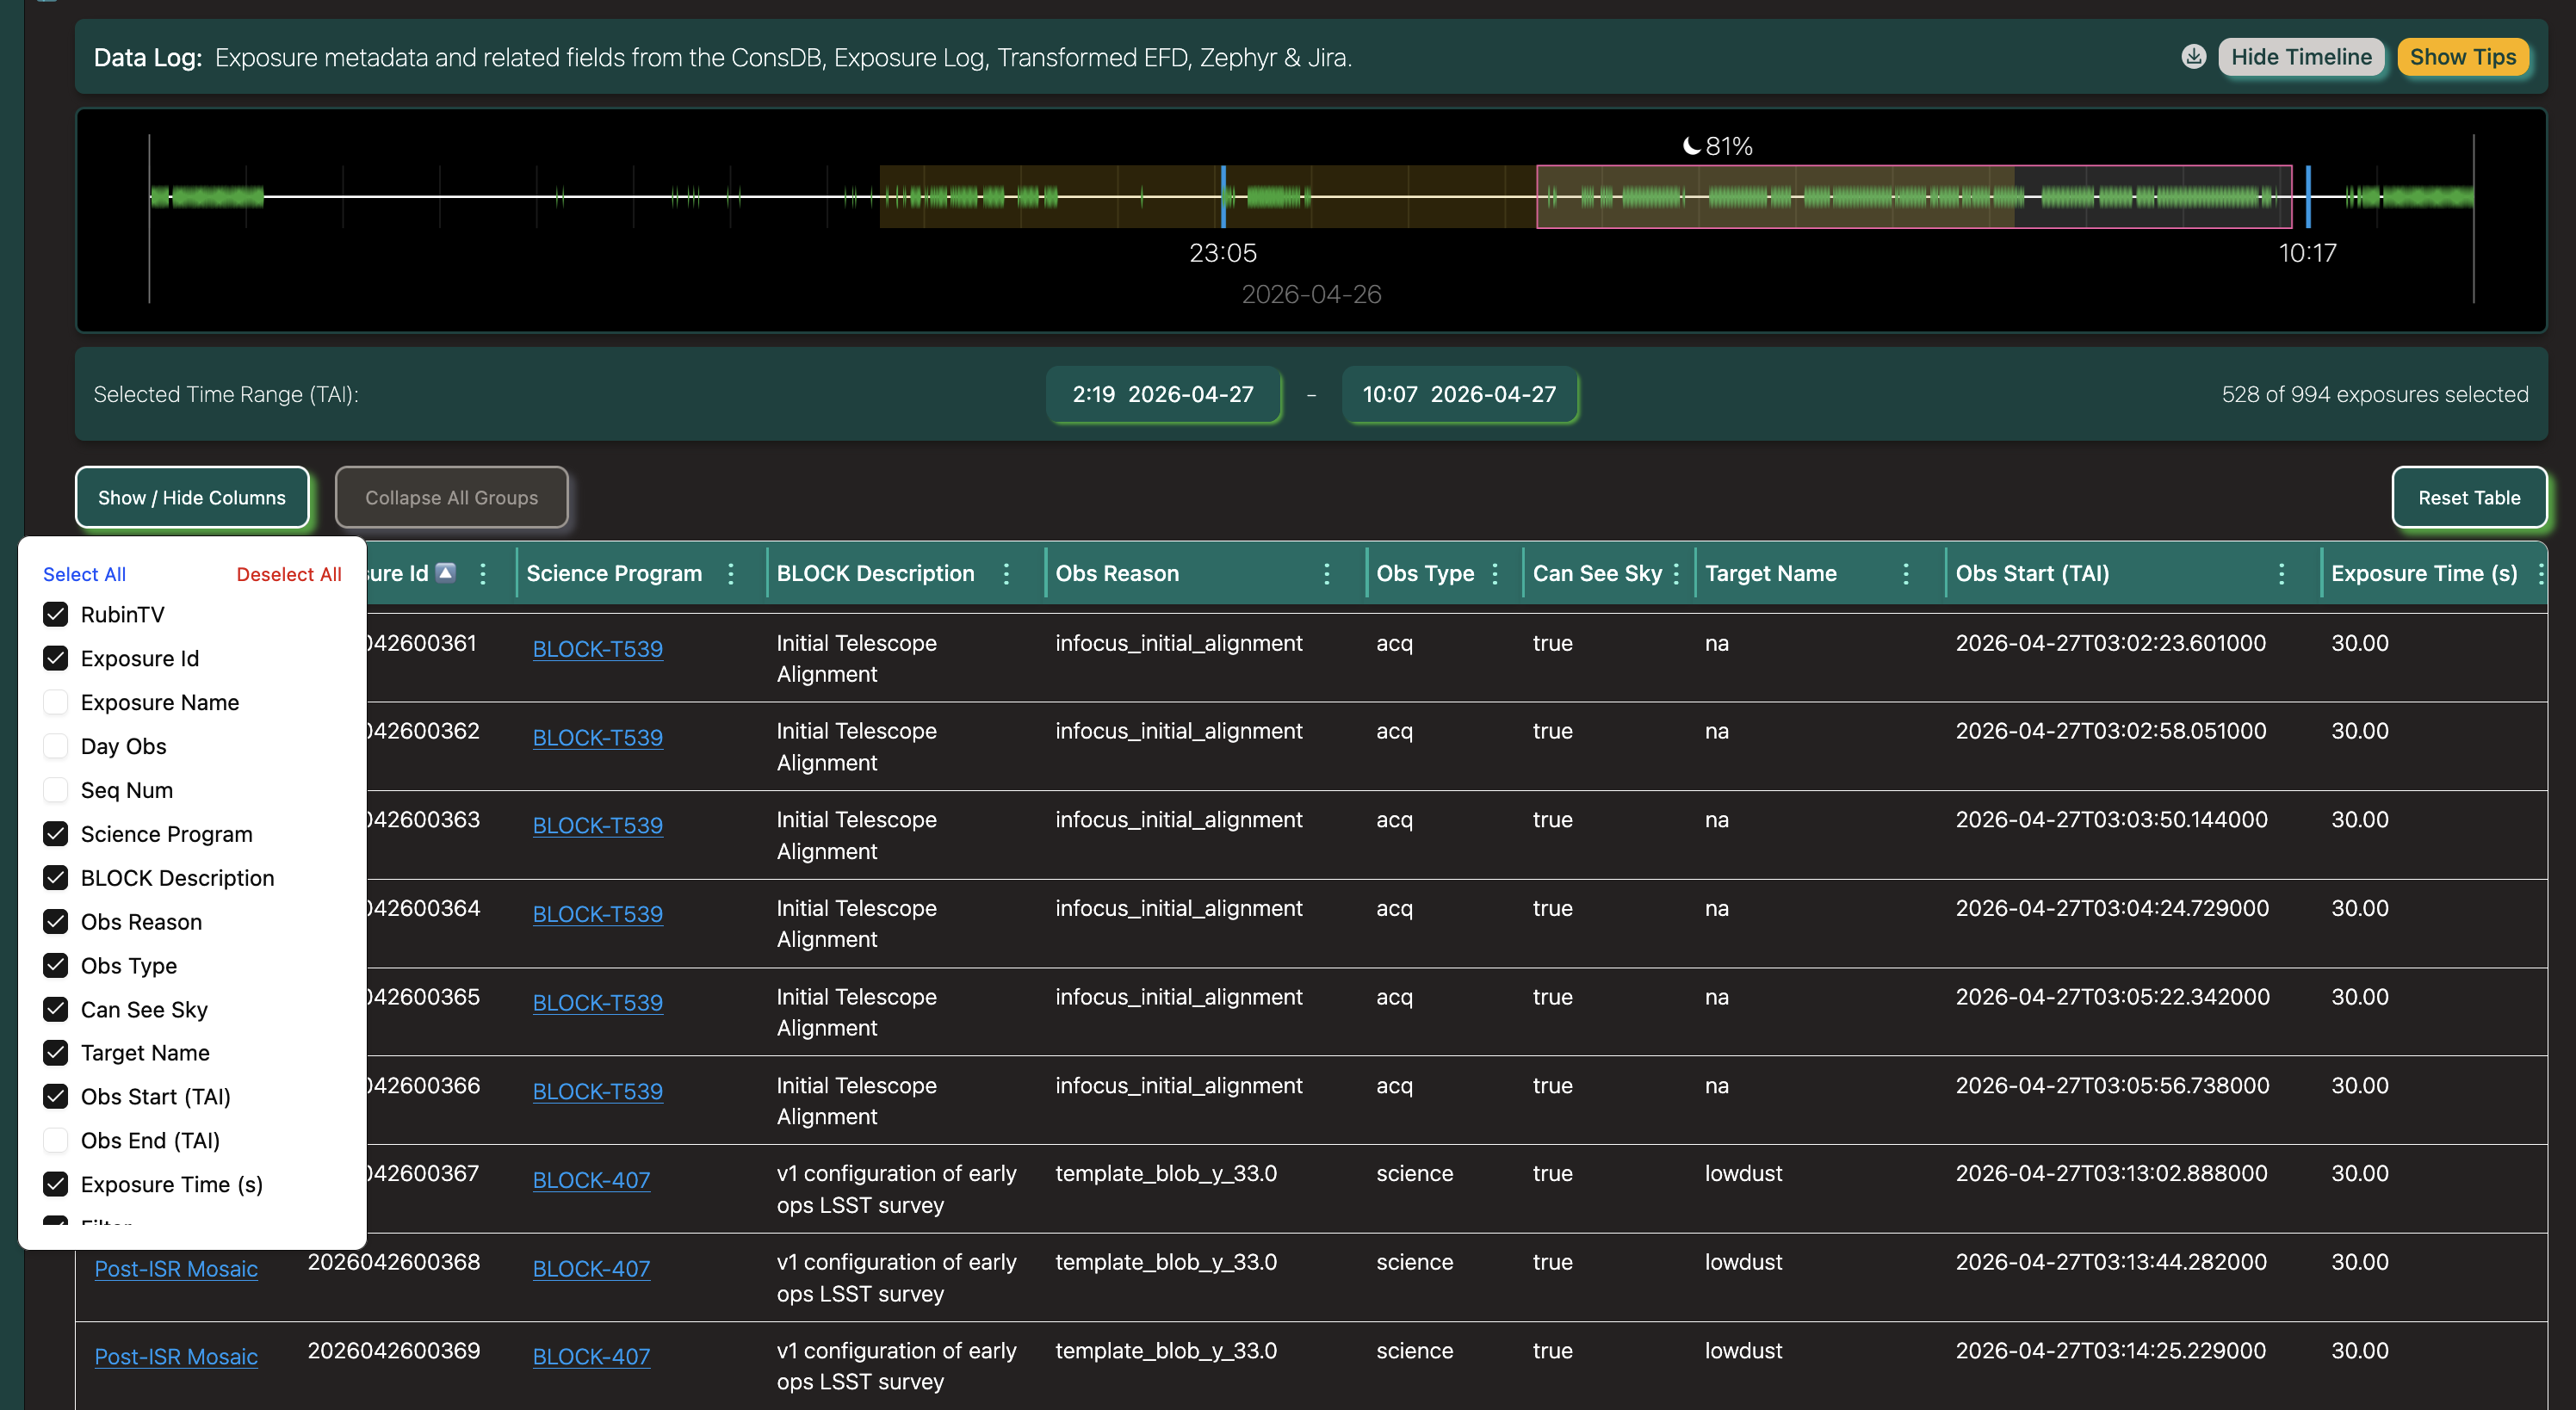
\includegraphics[height=8cm]{images/data-log-columns-short.png}
   \end{tabular}
   \end{center}
   \caption[example]
   { \label{fig:datalogcols}
The Data Log table invites users to select all columns of metadata associated to the
exposures, or only the columns of their interest.}
   \end{figure}

     \begin{figure} [ht]
   \begin{center}
   \begin{tabular}{c} %% tabular useful for creating an array of images
   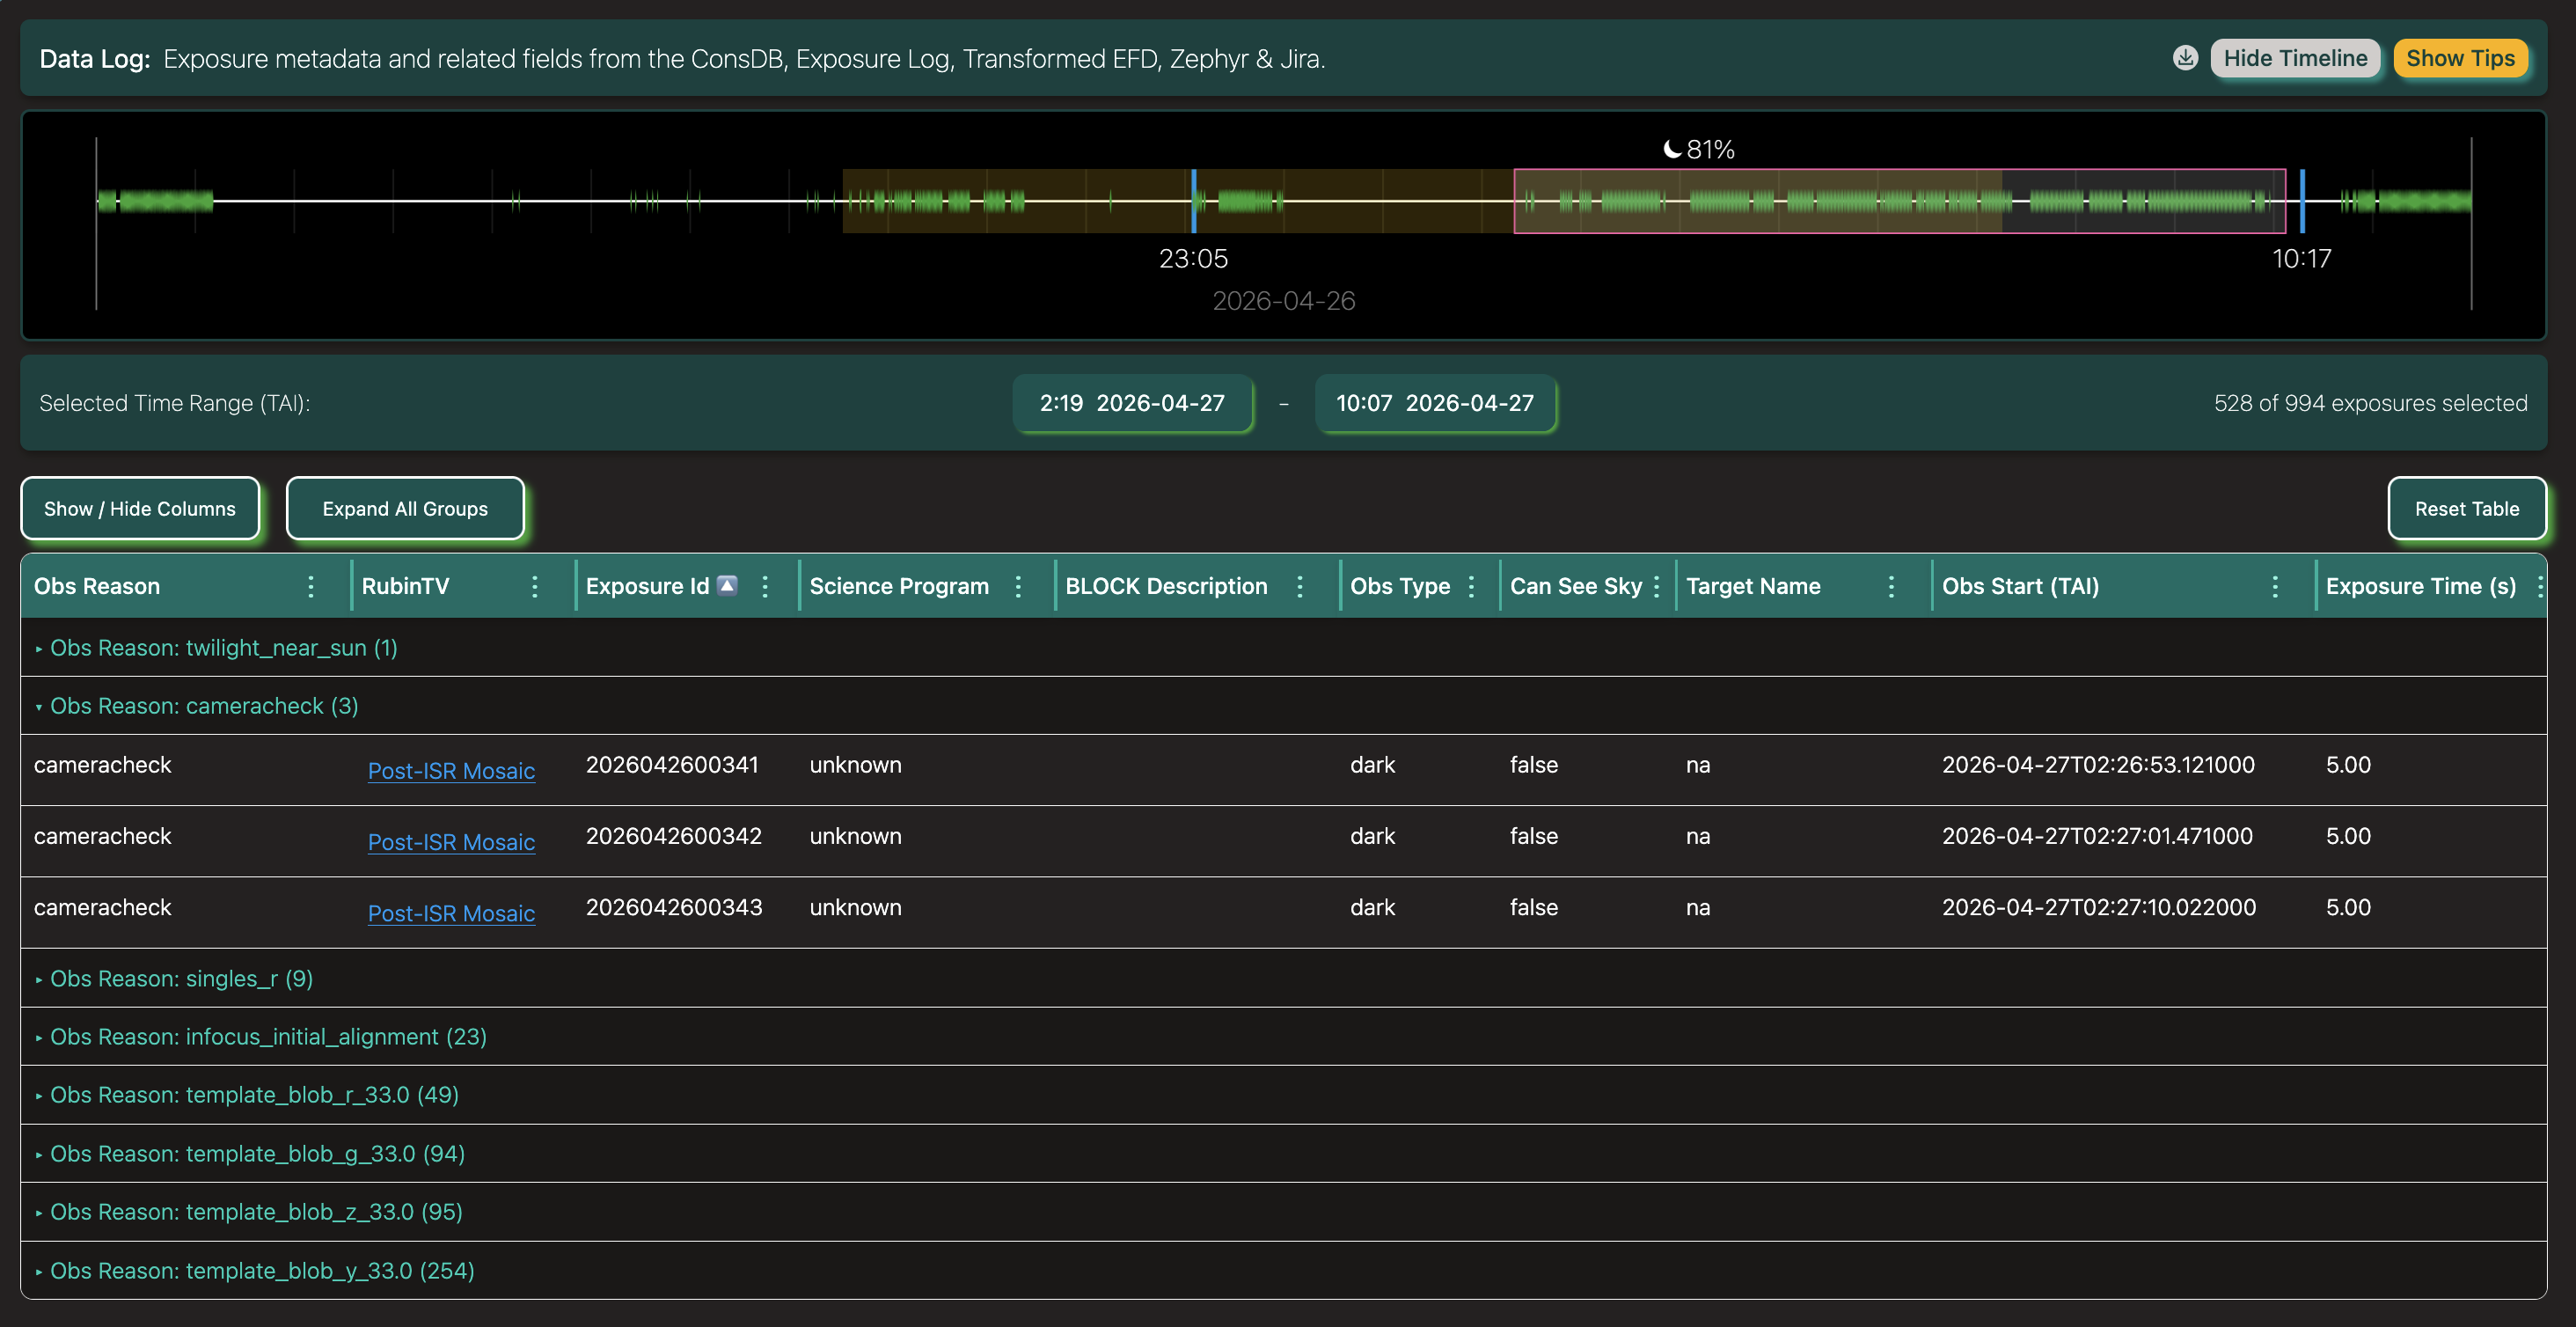
\includegraphics[height=8cm]{images/data-log-group-short.png}
   \end{tabular}
   \end{center}
   \caption[example]
   { \label{fig:dataloggroup}
The Data Log table allows grouping based on the data available in any of the selected
columns for unique filtering and searching.}
   \end{figure}

\FloatBarrier
\subsection{Context Feed}
\label{sec:contextfeed}

Before integration to the Nightly Digest, the Context Feed page had a predecessor: ROLEX
\cite{Ribeiro-Rolex}. ROLEX, or Rubin Observatory Log EXplorer, is a logging display that integrates
telemetric and narrative data for observatory specialists and commissioning scientists. By
viewing Narrative Log entries alongside script configurations and errors, users gain a clear
understanding of the Observing Specialists' activities over the course of an observation day.

The Context Feed page [Fig ~\ref{fig:contextfeed}] is an iteration on this integrated data visualization through
development collaboration with the survey scheduler team. This page expands on the
Observing Specialists’ written summary in the Night Report applet [Fig ~\ref{fig:nightreport}] and the Time Accounting
applet [Fig ~\ref{fig:timeacc}], to add detail to events that occurred during the available observing time and
elaborate on what was happening during different categories shown in the Time Accounting
applet. The Context Feed takes telemetric data from the EFD to include scripts, faults,
and exposures and displays these chronologically with written log messages from the
Observing Specialists in the Narrative Log. Combining this data into a timeline and a
table to display events and their descriptions allows the user to imagine themselves
shadowing the Observing Specialists during the observation day. From the Context Feed we
can understand what the Observing Specialists wrote about their activities, what scripts
and programmatic actions were taken, their results, details of any faults, and
how the Observing Specialists and observatory components reacted. Crucially, when an operational
anomaly or fault is logged, users can isolate the event within the feed to instantly extract
the specific system error messages while simultaneously reviewing the surrounding script configurations
and real-time operator remarks to determine the exact conditions that triggered the failure.

  \begin{figure} [ht]
   \begin{center}
   \begin{tabular}{c} %% tabular useful for creating an array of images
   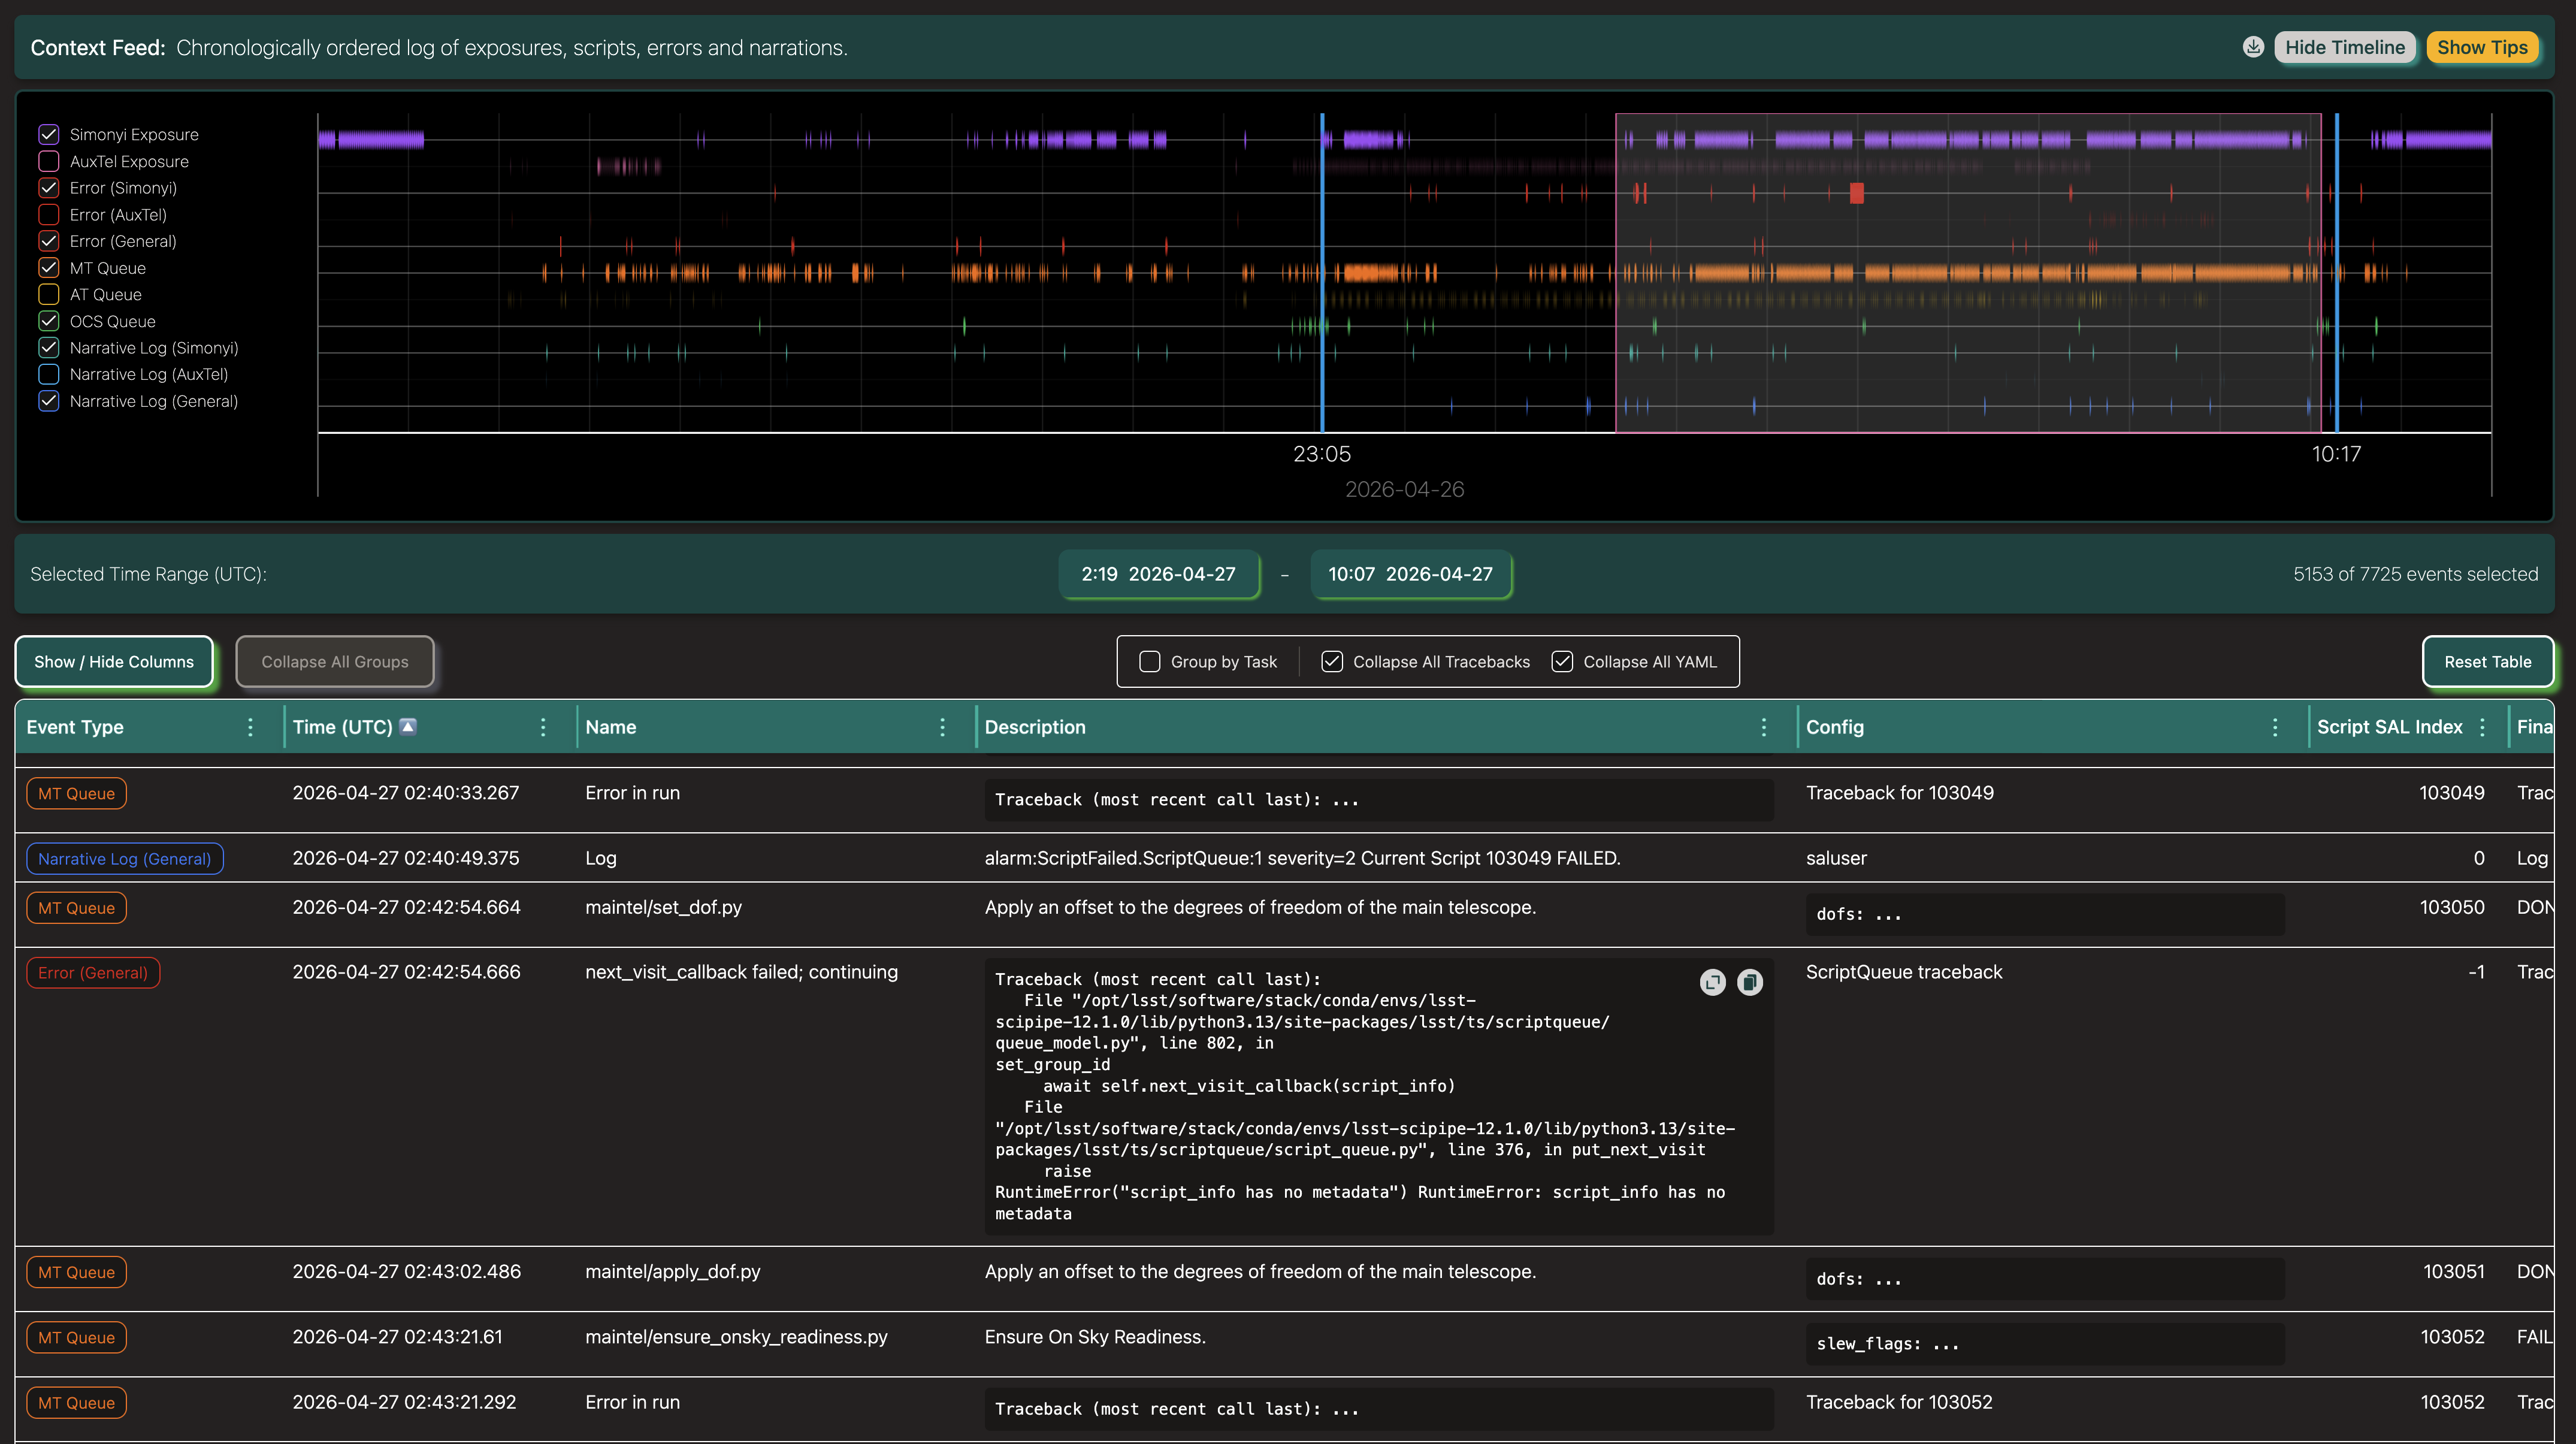
\includegraphics[height=9.75cm]{images/context-feed-w-traceback.png}
   \end{tabular}
   \end{center}
   \caption[example]
   { \label{fig:contextfeed}
The Context Feed page displays a timeline of events by each type, then displays a table of
these below, expanding on each category by displaying different attributes including
script configurations, messages, and telemetric timestamps.}
   \end{figure}

   \FloatBarrier
\subsection{Visit Maps}
\label{sec:vmp}

The Visit Maps page [Fig ~\ref{fig:vmp}] expands on the main summary page’s Visit Map applet [Fig ~\ref{fig:vma}]
to give a larger and more detailed view of the visits taken during the selected observation day range.
This visualization was a result of our cross disciplinary work with the survey scheduler team who creates these maps to
evaluate survey progress. With their help, we offer a larger view of the visits on a
planispheric projection and is also visualized with an armillary projection adjacent.
Both projections work together; as the user slides the time control through the
available time range, the visits populate on both maps simultaneously. The data
populating these plots is accessed via ConsDB and added by our almanac data. These
detailed projections show additional data to contextualize the Visit Map data being
shown: the planned final depth of LSST survey\cite{2019ApJ...873..111I}, the moon and sun coordinates, the
ecliptic, the plane of the Milky Way, the horizon, and the zenith distance of 70
degrees.

  \begin{figure} [ht]
   \begin{center}
   \begin{tabular}{c} %% tabular useful for creating an array of images
   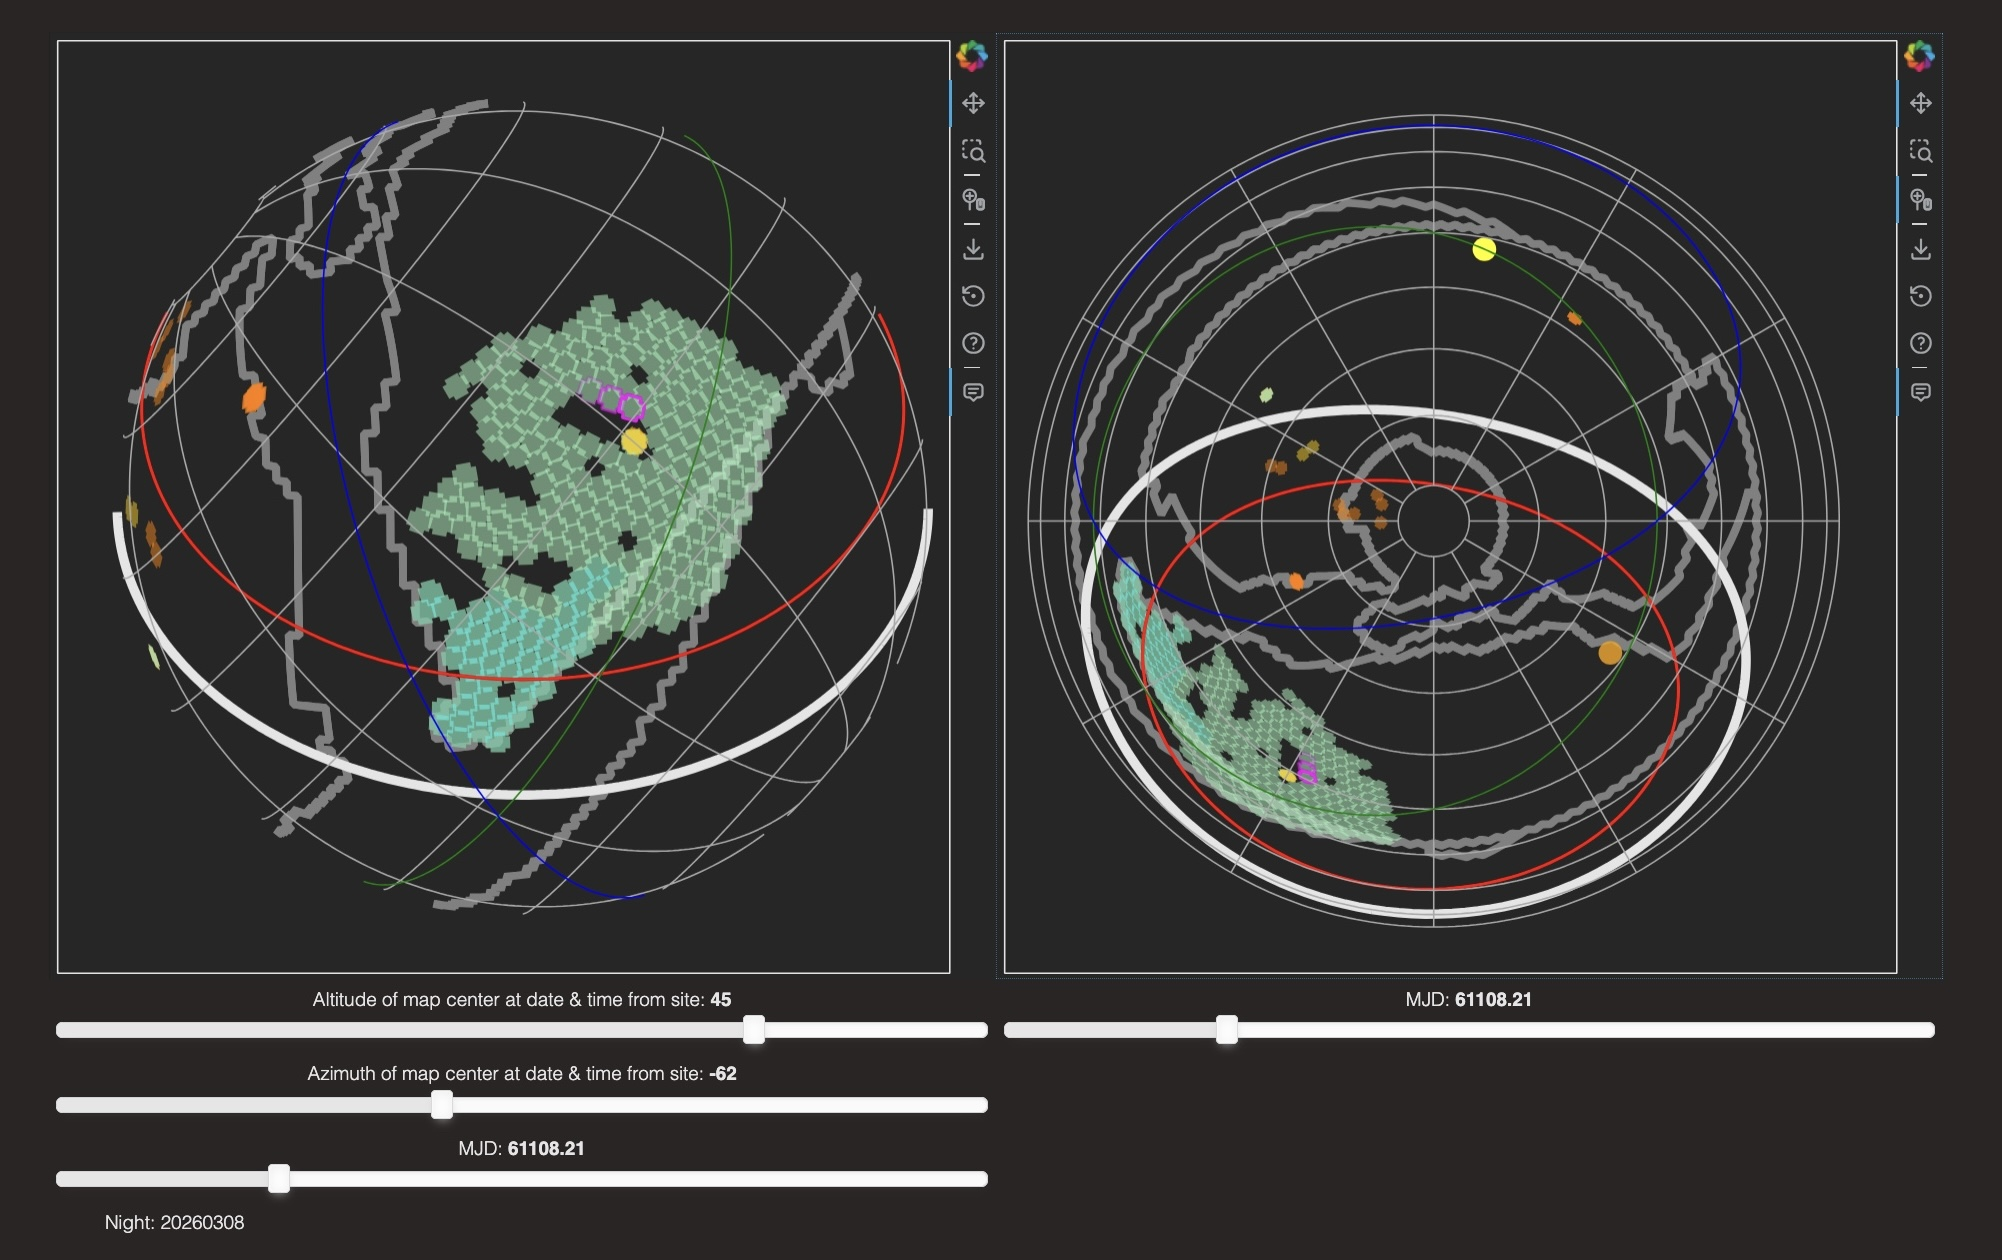
\includegraphics[height=10cm]{images/visit-map-page.jpg}
   \end{tabular}
   \end{center}
   \caption[example]
   { \label{fig:vmp}
The Visit Map page displays larger versions of the planispheric and armillary projections
of the exposures taken during the time frame with additional sliders to navigate the
data.}
   \end{figure}

\FloatBarrier
\section{Future Improvements}

The Nightly Digest continues to be improved upon as we work with Observing
Specialists, summit support staff, and project scientists to understand their
evolving needs as Rubin Observatory moves through commissioning and into operations.
One major feature in development is the automation of a unified Observatory Status,
with input from Observing Specialists. This new control system feature has been
integrated with the Observing Specialists’ interface LOVE and the scheduling
component of the control software. With this new telemetry data collected from the EFD
 the Nightly Digest will improve the way we report and visualize our
 Time Accounting applet [Fig ~\ref{fig:timeacc}], Time Loss card,
 and our in-development Time Loss page. This information will be automatically time
 based and serves as another use of a timeline, specifically that users would like to see on our main summary page.

Timelines have become increasingly popular with our users and we continue to arrange
our visualizations to include them in more pages that would leverage a timeline-based display,
as they have recently been added to our Data Log page. We continue to solicit feedback from
our user base and work to integrate and unify the different logging tools that each team uses,
so that Nightly Digest may become a launching pad towards more detailed debugging tools.
A prominent upcoming priority is the implementation of automated report generation built
directly from the metrics summarized within the dashboard. Developing a minimum useful
product for these operational reports will allow technical leads and stakeholders to
easily export and share high-level summaries of a given observing window.

Our future milestones prioritize user experience and performance tuning to make the
dashboard more performant, fully include AuxTel’s data across all application pages,
and evaluate the long-term scope of the platform's availability. While the Nightly Digest
is currently optimized as a project-internal tool for engineering and summit diagnostics,
future operational phases will determine whether to maintain this internal focus or
adapt elements of the dashboard for wider community access.

  \begin{figure} [ht]
   \begin{center}
   \begin{tabular}{c} %% tabular useful for creating an array of images
   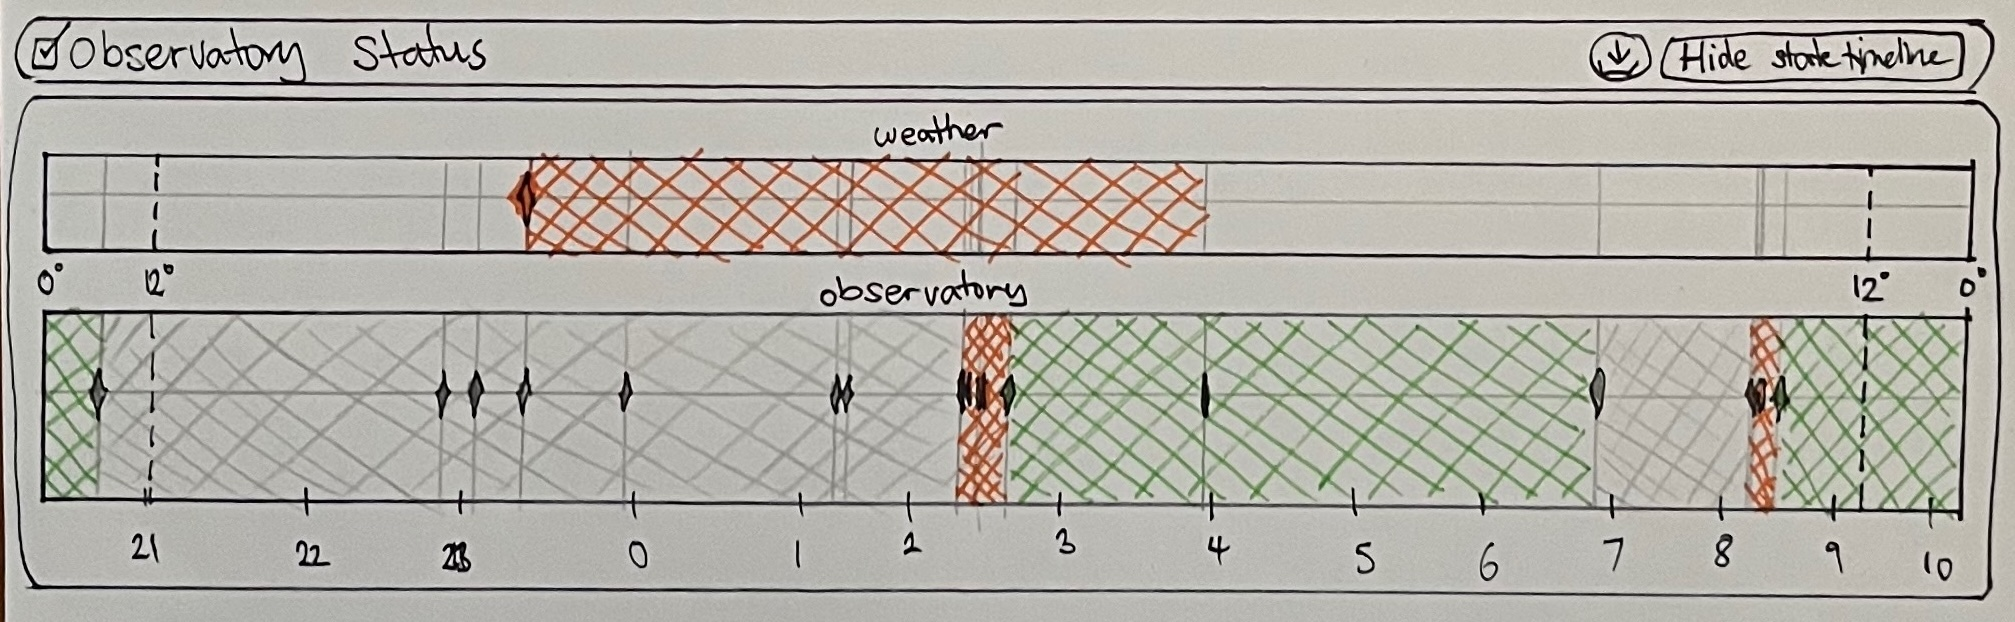
\includegraphics[height=5cm]{images/timeline_w_weather.jpeg}
   \end{tabular}
   \end{center}
   \caption[example]
   { \label{fig:drawtimeline}
Hand drawn designs for Observatory Status timeline and applet to show the design process
and many ideas are developed while only some make it into the application.}
   \end{figure}

     \begin{figure} [ht]
   \begin{center}
   \begin{tabular}{c} %% tabular useful for creating an array of images
   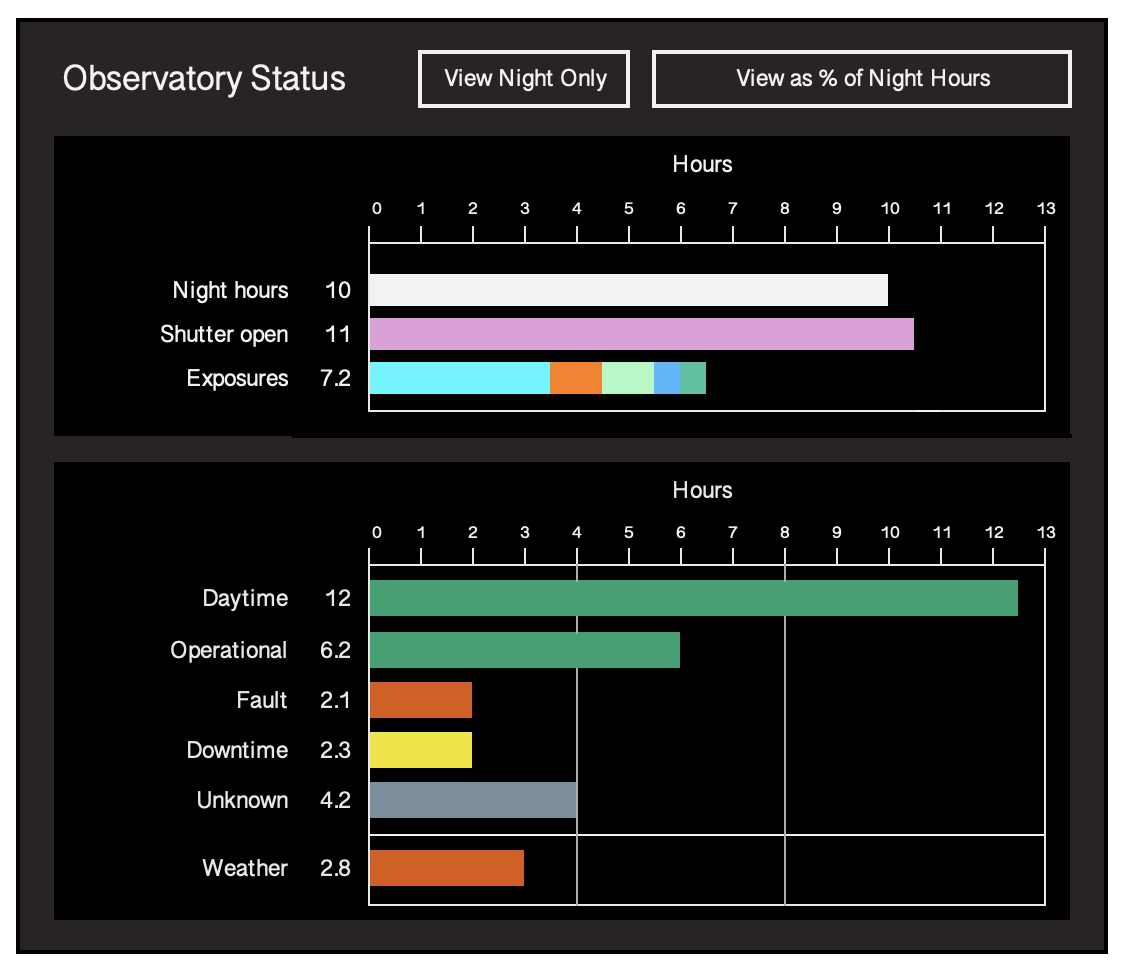
\includegraphics[height=5cm]{images/timeaccbar.png}
   \end{tabular}
   \end{center}
   \caption[example]
   { \label{fig:barside}
Digitally created models of each applet are used to visualize the color scheme before
finalizing the designs, as shown here in this time accounting horizontal bar chart.}
   \end{figure}

\FloatBarrier
\section{Conclusion}

In the past two years, the logging team and Nightly Digest application have made
significant steps towards unifying the electronic logging landscape at Rubin Observatory.
Users now have a landing page to understand the progress and status of the previous
nights’ observing time, and look back to compare with other time periods. Questions about
exposure volume, quality and efficiency of exposures taken, context around operations, and
information about interruptions can now be easily identified and understood by technical
and scientific audiences. The Nightly Digest continues to be improved based on user
feedback and integrates developing systems to support summit staff and Rubin Observatory
operations.
